\documentclass[11pt,a4paper]{article}

\usepackage[margin=1in]{geometry}
\usepackage{amsmath,amssymb,amsthm}
\usepackage{cancel}
\usepackage{booktabs,longtable,array}
\usepackage[expansion=false]{microtype}
\usepackage{xcolor}
\usepackage{graphicx}
\usepackage{enumitem}
\usepackage{listings}
\usepackage{tikz}
\usepackage{caption}
\usepackage{fancyhdr}
\usepackage{titlesec}
\usepackage[colorlinks=true,linkcolor=BlueLink,citecolor=BlueLink,urlcolor=BlueLink]{hyperref}

\usetikzlibrary{arrows.meta,positioning,calc,decorations.pathmorphing,patterns}

\definecolor{BlueLink}{HTML}{1A4F8C}
\definecolor{CodeBg}{HTML}{F6F7F9}
\definecolor{CodeKw}{HTML}{8B1A6B}
\definecolor{CodeCm}{HTML}{5A7D5A}
\definecolor{BoxBg}{HTML}{F0F4F8}
\definecolor{WarnBg}{HTML}{FDF3E7}
\definecolor{WarnRule}{HTML}{C87A2A}
\definecolor{GoodRule}{HTML}{2E7D5B}
\definecolor{Gray60}{HTML}{666666}

\lstset{
  basicstyle=\ttfamily\footnotesize, backgroundcolor=\color{CodeBg},
  keywordstyle=\color{CodeKw}\bfseries, commentstyle=\color{CodeCm}\itshape,
  stringstyle=\color{GoodRule}, frame=leftline, framerule=1.2pt,
  rulecolor=\color{BlueLink}, framesep=8pt, xleftmargin=10pt,
  breaklines=true, showstringspaces=false, language=Python, numbers=none,
}

\newcommand{\code}[1]{\texttt{\small #1}}
\newcommand{\R}{\mathbb{R}}
\newcommand{\E}{\mathbb{E}}
\newcommand{\bx}{\mathbf{x}}
\newcommand{\bu}{\mathbf{u}}
\newcommand{\bp}{\mathbf{p}}
\newcommand{\bv}{\mathbf{v}}
\newcommand{\ba}{\mathbf{a}}

\newtheorem{theorem}{Theorem}
\newtheorem{proposition}[theorem]{Proposition}

\newenvironment{keybox}{%
  \par\medskip\noindent
  
\begin{tikzpicture}\node[fill=BoxBg,draw=BlueLink,line width=1pt,rounded corners=2pt,
    inner sep=10pt,text width=\dimexpr\linewidth-24pt\relax,align=justify]\bgroup}
  {\egroup;\end{tikzpicture}\par\medskip}

\newenvironment{warnbox}{%
  \par\medskip\noindent
  
\begin{tikzpicture}\node[fill=WarnBg,draw=WarnRule,line width=1pt,rounded corners=2pt,
    inner sep=10pt,text width=\dimexpr\linewidth-24pt\relax,align=justify]\bgroup}
  {\egroup;\end{tikzpicture}\par\medskip}

\titleformat{\section}{\Large\bfseries\color{BlueLink}}{\thesection}{0.7em}{}
\titleformat{\subsection}{\large\bfseries}{\thesubsection}{0.6em}{}

\emergencystretch=1.2em

\pagestyle{fancy}
\fancyhf{}
\fancyhead[L]{\footnotesize\color{Gray60} Kinodynamic Multi-Robot Navigation with RL}
\fancyhead[R]{\footnotesize\color{Gray60}\thepage}
\renewcommand{\headrulewidth}{0.4pt}

\title{\vspace{-1.5cm}\textbf{The Robot That Cannot Stop}\\[0.25cm]
\large Kinodynamic Multi-Robot Navigation with Reinforcement Learning\\[0.15cm]
\normalsize An account of what we built, what it does, and what it taught us}
\author{\normalsize Project \code{kinodynamic\_rl} \quad$\cdot$\quad branch \code{aditya}}
\date{\normalsize 27 August 2026}

\begin{document}
\maketitle
\thispagestyle{empty}

\begin{keybox}
\textbf{How to read this.} It is written as one continuous account rather than a set of
reference entries. Parts I--V tell the story in order: the physical problem, how we turned
it into something a learning algorithm can consume, the idea we are testing, what the
experiments actually said, and where it goes. Theory appears at the point where the
practical work needs it, not before.

\textbf{Assumed background.} Comfort with calculus, linear algebra and probability.
\emph{No} reinforcement learning or motion planning is assumed --- every piece of machinery
used is derived here.

\textbf{Reference material} --- the exact input/output contracts, which library owns which
decision, the hyperparameter table, the source map and the reading list --- is in the
appendices, so that the narrative does not stop to look things up.

\textbf{On sourcing.} Every number is read from \code{src/}, \code{conf/} or
\code{experiments/}. Claims we have not verified are marked as such, in place. This
document also records the things we got \emph{wrong}; Part IV is largely about those.
\end{keybox}

\tableofcontents
\newpage

\part{The Problem}

%======================================================================
\section{A Robot That Cannot Stop}
%======================================================================

Start with the machine, because everything else follows from it.

Our robot is a \emph{second-order unicycle}. It has a position, a heading, a forward speed
and a turn rate --- five numbers,
\[
  \bx = (x,\; y,\; \theta,\; v,\; \omega) \in \R^5,
\]
and you do not get to set any of them directly. What you get to set is
\emph{acceleration}:
\[
  \bu = (a,\;\alpha) \in \R^2,
  \qquad
  \dot x = v\cos\theta,\quad
  \dot y = v\sin\theta,\quad
  \dot\theta = \omega,\quad
  \dot v = a,\quad
  \dot\omega = \alpha .
\]

The parameters are not ours. They come verbatim from the \textbf{dynobench} model
\code{unicycle2\_v0}, which is what the db-CBS planning benchmarks reference:

\begin{center}
\begin{tabular}{llr}
\toprule
Symbol & Meaning & Value \\
\midrule
$v_{\max}$      & max forward speed          & $0.5\ \text{m/s}$ \\
$v_{\min}$      & max reverse speed          & $-0.5\ \text{m/s}$ \\
$\omega_{\max}$ & max turn rate              & $0.5\ \text{rad/s}$ \\
$a_{\max}$      & max forward acceleration   & $0.25\ \text{m/s}^2$ \\
$\alpha_{\max}$ & max angular acceleration   & $0.25\ \text{rad/s}^2$ \\
body            & box (forward $\times$ lateral) & $0.5 \times 0.25\ \text{m}$ \\
\bottomrule
\end{tabular}
\end{center}

Two numbers fall out of that table and they run the rest of this document.

\begin{keybox}
\textbf{Braking distance.} Going from top speed to a standstill takes
$v_{\max}/a_{\max} = 2$ seconds, and in those two seconds the robot travels
\[
  d_{\text{brake}} \;=\; \frac{v_{\max}^2}{2a_{\max}} \;=\; \frac{0.5^2}{2(0.25)} \;=\; 0.50\ \text{m}.
\]

\textbf{Turning radius.} At top speed with maximum turn rate,
$\rho = v_{\max}/\omega_{\max} = 1.00$ m.
\end{keybox}

Sit with $d_{\text{brake}} = 0.5$ m for a moment. The robot's own body is $0.5$ m long. The
goal tolerance it will be asked to hit is $0.2$ m. So the distance this machine needs
\emph{merely to stop} is a full body length, and two and a half times the precision
demanded of it.

That is the entire problem. It is a sluggish machine, and a sluggish machine has to decide
what to do about an obstacle long before it arrives.

\subsection{The scenario}

Two of these robots, in an empty $5 \times 5$ metre square, facing each other three metres
apart on the same line. Each must drive to where the other one currently is.

\begin{center}
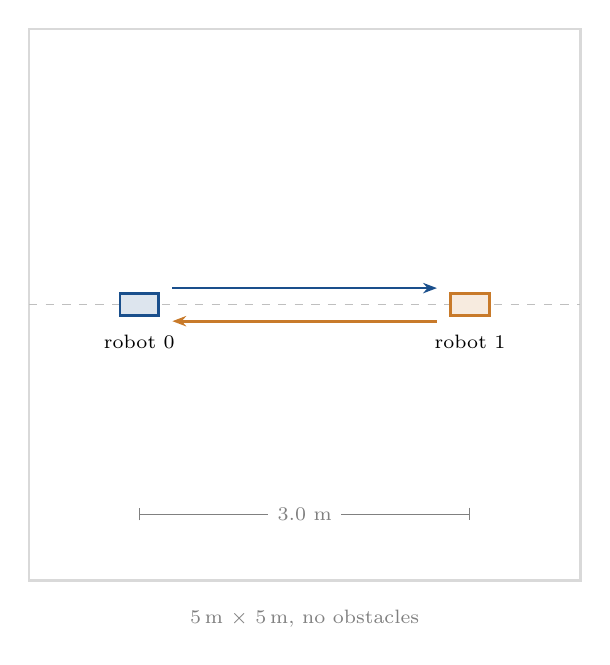
\begin{tikzpicture}[scale=1.4]
  \draw[gray!30,line width=1pt] (0,0) rectangle (5,5);
  \draw[gray!50,dashed] (0,2.5) -- (5,2.5);
  \node[draw=BlueLink,fill=BlueLink!15,line width=1pt,minimum width=14pt,minimum height=8pt]
       (r1) at (1,2.5) {};
  \node[draw=WarnRule,fill=WarnRule!15,line width=1pt,minimum width=14pt,minimum height=8pt]
       (r2) at (4,2.5) {};
  \node[below=3pt of r1,font=\scriptsize] {robot 0};
  \node[below=3pt of r2,font=\scriptsize] {robot 1};
  \draw[-{Stealth[length=5pt]},BlueLink,line width=1pt] (1.3,2.65) -- (3.7,2.65);
  \draw[-{Stealth[length=5pt]},WarnRule,line width=1pt] (3.7,2.35) -- (1.3,2.35);
  \node[font=\scriptsize,gray] at (2.5,-0.35) {$5\,$m $\times\ 5\,$m, no obstacles};
  \draw[|-|,gray] (1,0.6) -- (4,0.6) node[midway,fill=white,font=\scriptsize] {$3.0$ m};
\end{tikzpicture}
\end{center}

We did not invent this either. It is \code{swap2\_unicycle2.yaml} from the db-CBS
benchmark, ported verbatim. Using a published instance rather than a hand-made one is a
guard against ourselves: a scenario you design yourself can be tuned, consciously or not,
until your method wins.

And notice what is missing from it. The robots are on the \emph{same line}. No lane offset,
no geometric asymmetry, nothing anywhere in the problem statement that says which robot
should go left and which should go right. Hold on to that. By Part IV it will turn out to
be the thing that matters most, and not for the reason we first thought.

%======================================================================
\section{Why the Literature Works First-Order}
%======================================================================

There is a large, successful body of work on learned multi-robot collision avoidance. Almost
all of it uses a \emph{first-order} model, in which the state is $(x,y,\theta)$ and the
control input is the velocity itself:
\[
  \text{\textbf{first order:}}\quad \dot x = v\cos\theta,\quad \dot y = v\sin\theta,\quad
  \dot\theta=\omega, \qquad \bu = (v,\omega).
\]

That is not a small modelling convenience. It changes what a decision \emph{is}.

\begin{center}
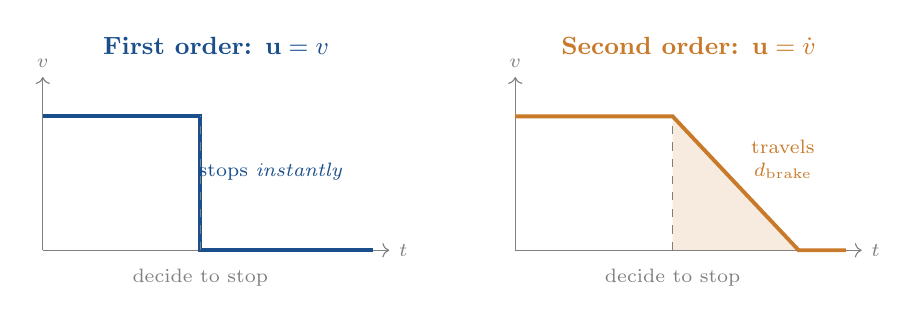
\begin{tikzpicture}[scale=1]
  \begin{scope}
    \node[font=\bfseries\small,BlueLink] at (2.2,2.6) {First order: $\bu = v$};
    \draw[->,gray] (0,0) -- (4.4,0) node[right,font=\scriptsize] {$t$};
    \draw[->,gray] (0,0) -- (0,2.2) node[above,font=\scriptsize] {$v$};
    \draw[BlueLink,line width=1.4pt] (0,1.7) -- (2,1.7) -- (2,0) -- (4.2,0);
    \draw[dashed,gray] (2,0) -- (2,1.7);
    \node[font=\scriptsize,BlueLink] at (2.9,1.0) {stops \emph{instantly}};
    \node[font=\scriptsize,gray] at (2,-0.35) {decide to stop};
  \end{scope}
  \begin{scope}[xshift=6cm]
    \node[font=\bfseries\small,WarnRule] at (2.2,2.6) {Second order: $\bu = \dot v$};
    \draw[->,gray] (0,0) -- (4.4,0) node[right,font=\scriptsize] {$t$};
    \draw[->,gray] (0,0) -- (0,2.2) node[above,font=\scriptsize] {$v$};
    \draw[WarnRule,line width=1.4pt] (0,1.7) -- (2,1.7) -- (3.6,0) -- (4.2,0);
    \draw[dashed,gray] (2,0) -- (2,1.7);
    \fill[WarnRule,opacity=0.15] (2,0) -- (2,1.7) -- (3.6,0) -- cycle;
    \node[font=\scriptsize,WarnRule,align=center] at (3.4,1.15) {travels\\$d_{\text{brake}}$};
    \node[font=\scriptsize,gray] at (2,-0.35) {decide to stop};
  \end{scope}
\end{tikzpicture}
\end{center}

For a first-order robot, ``decide to stop'' and ``stopped'' are the same instant. For ours
they are separated by two seconds, and in that gap the robot sweeps out the shaded triangle
of area $v^2/(2a_{\max})$. Every difficulty in this project is that triangle.

Two consequences deserve names, because we will keep returning to them.

\begin{keybox}
\textbf{The value function depends on velocity.} For a first-order robot, ``where am I''
is $(x,y,\theta)$ and that fully determines how long the rest of the task takes. For ours it
does not: sitting at a point at $v=0.5$ pointed \emph{at} the goal and sitting at the same
point at $v=0.5$ pointed \emph{away} from it are entirely different situations. Position
alone no longer determines cost-to-go. \emph{Part III turns this observation into the
contribution.}

\textbf{Some states are already lost.} A first-order robot can always avoid a collision by
commanding $v=0$. Ours cannot. Thirty centimetres from a wall at $0.5$ m/s pointed
straight at it, no admissible control sequence avoids the impact --- it needs fifty. Such
states are called \textbf{inevitable collision states} (ICS), and they exist only in the
second-order world. \emph{Part IV uses them to kill one of our own hypotheses.}
\end{keybox}

\subsection{The gap, stated precisely}

We checked this rather than assumed it, by reading the action-space definitions in the
primary papers.

\begin{center}
\small
\begin{tabular}{p{4.2cm}p{4.0cm}p{5.4cm}}
\toprule
\textbf{Work} & \textbf{Method} & \textbf{Action space} \\
\midrule
Long et al., ICRA 2018 \newline (\code{arXiv:1709.10082})
  & decentralised deep RL & ``a set of permissible \emph{velocities}'' --- first order \\
\addlinespace
Fan et al., IJRR \newline (\code{arXiv:1808.03841})
  & decentralised deep RL & velocity commands --- first order \\
\addlinespace
db-CBS, K-CBS, K-ARC
  & search-based planning & full second-order dynamics, \emph{no learning} \\
\bottomrule
\end{tabular}
\end{center}

So: the people who learn work first-order, and the people who handle second-order dynamics
do not learn. \textbf{Decentralised reinforcement learning under genuine second-order
dynamics is close to unoccupied ground.} That is the opening this project aims at, and it
is the reason the work is worth doing even when --- as Part IV will show --- the headline
experiment fails.
\part{Turning a Robot Into a Learning Problem}

%======================================================================
\section{What Reinforcement Learning Demands}
%======================================================================

Before handing this robot to a learning algorithm we should say what such an algorithm
actually wants from us. The answer is a short list, but each item has a catch.

\subsection{The contract: a Markov Decision Process}

An MDP is five things:

\begin{center}
\small
\begin{tabular}{clp{9.4cm}}
\toprule
& \textbf{Item} & \textbf{What it means, in our case} \\
\midrule
$\mathcal S$ & states     & Every situation the world can be in. Ours: five numbers per robot. \\
$\mathcal A$ & actions    & Every choice available. Ours: a pair of accelerations. \\
$P$          & transitions& Given a situation and a choice, what happens next. Ours: the equations of motion. \\
$R$          & reward     & A single number after each step saying how that went. \\
$\gamma$     & discount   & How much we care about later rewards versus sooner ones. \\
\bottomrule
\end{tabular}
\end{center}

Four of those we supply in Section~\ref{sec:env}. The fifth, $\gamma$, is not really the
world's business at all --- it is a statement about \emph{us} --- and that turns out to
matter (\S\ref{sec:gammabug}).

\subsection{The one real requirement: the Markov property}

The demand hiding inside ``$P$'' is this: \textbf{the next situation must depend on the
current one and the current choice, and on nothing else.} No dependence on how you got here.
The present must be a complete summary of the past.

Why insist? Because otherwise the agent's job is impossible to state. If ``what happens
next'' depends on something the agent cannot see --- three steps of history, a hidden
variable --- then no rule of the form ``look at the situation, choose an action'' can be
optimal, because the same-looking situation sometimes wants different actions.

\begin{keybox}
\textbf{Physics hands us this for free, and it is worth appreciating why.} Our equations of
motion are a \emph{first-order} differential equation: every derivative on the left is a
first derivative, and the right side mentions only $\bx$ itself. So $\bx$ at this instant
determines $\bx$ at the next instant. Where the robot has \emph{been} is irrelevant --- only
where it is and how fast it is going.

Note this is a claim about $\bx = (x,y,\theta,v,\omega)$, not about position. Position alone
is \emph{not} Markov for our robot: knowing you are at $(2,3)$ tells you nothing about where
you will be in a tenth of a second unless you also know $v$ and $\theta$. That is exactly
why the state carries velocity, and --- as Section~\ref{sec:braking} argues --- exactly why
a potential that ignores velocity is the wrong potential.
\end{keybox}

\subsection{What we want: a policy, and what it is worth}

A \textbf{policy} $\pi$ is the thing we are trying to learn: a rule that looks at a situation
and produces an action. We write $\pi(a \mid s)$ and read it ``the probability of choosing
action $a$ when in situation $s$''.

Why a probability rather than a definite choice? Two reasons. During learning the agent
\emph{must} try things it is unsure about, and randomness is how it does that. And once
learned, a random policy is also a mathematically convenient object --- as
Section~\ref{sec:pg} shows, you can differentiate a probability, which is what makes
gradient-based learning possible at all.

Now, how good is a policy? Not ``what reward did it get this step'' --- that is short-sighted,
and slamming into a wall at speed feels fine right up until it does not. What we want is the
\textbf{total reward from here onward}:
\begin{equation}
\label{eq:value}
V^\pi(s) \;=\; \E_\pi\!\left[\underbrace{r_0 + \gamma r_1 + \gamma^2 r_2 + \gamma^3 r_3 + \cdots}_{\text{all future reward, discounted}} \;\Big|\; s_0 = s\right].
\end{equation}
Read it left to right: \emph{starting from situation $s$ and following policy $\pi$, add up
every reward you will ever collect, shrinking each one a little more the further off it is.}
The $\E$ says ``on average'', because the policy and possibly the world are random.

The close relative $Q^\pi(s,a)$ is the same quantity but with the first action forced to be
$a$: \emph{what is it worth to do $a$ right now, and behave normally afterwards?} The
difference between $Q$ and $V$ is the whole basis of learning, and Section~\ref{sec:pg}
returns to it.

\subsection{Why shrink the future at all?}

The factor $\gamma$ raised to increasing powers is doing something specific and it is worth
being concrete about what.

\begin{center}
\small
\begin{tabular}{lrl}
\toprule
\textbf{Reward arriving in\ldots} & \textbf{is multiplied by} & \\
\midrule
1 step ($0.1$\,s)   & $0.99$   & \\
10 steps ($1$\,s)   & $0.904$  & barely discounted \\
50 steps ($5$\,s)   & $0.605$  & \\
100 steps ($10$\,s) & $0.366$  & worth a third of the same reward now \\
300 steps ($30$\,s) & $0.049$  & the full episode --- almost worthless \\
\bottomrule
\end{tabular}
\end{center}

Two motives. \emph{Mathematically}, without shrinking, an infinite stream of rewards adds up
to infinity and comparing two infinite policies is meaningless. \emph{Practically}, $\gamma$
sets how far ahead the agent bothers to look. The standard summary is
\[
  \frac{1}{1-\gamma} \;=\; \frac{1}{0.01} \;=\; 100\ \text{steps} \;=\; 10\ \text{seconds}.
\]

\begin{warnbox}
\textbf{Our episode is 30 seconds long and our agent's horizon is 10.} The table above says
a reward at the end of the episode is worth $4.9\%$ of the same reward now. So the
\emph{agent is deliberately near-sighted relative to its own task} --- it can barely see the
end of the episode from the start.

That is not obviously wrong --- most of what matters in navigation is local --- but it is a
choice, and for a robot whose defining feature is that it must act early it deserves more
scrutiny than it has received. Nobody has swept $\gamma$ on this problem.
\end{warnbox}

\subsection{The equation we would love to solve, and cannot}

Suppose you already knew the best possible value of every situation --- call it $V^*$. Then
acting well would be trivial: try each action, see which one leads somewhere with the highest
value, do that. This self-consistency is the \textbf{Bellman optimality equation}:
\begin{equation}
\label{eq:bellman}
V^*(s) \;=\; \max_{a}\ \E_{s'\sim P(\cdot|s,a)}\big[\underbrace{R(s,a,s')}_{\text{reward now}} + \underbrace{\gamma V^*(s')}_{\text{discounted value of where you land}}\big].
\end{equation}

In words: \emph{the best you can do from here is the best over your available actions of
(what you get immediately, plus a discounted version of the best you can do from wherever
that puts you).} It is almost a tautology, and that is its strength --- it must be true, so
any $V$ satisfying it everywhere \emph{is} the answer.

So why not just solve it? For a small finite problem you can: sweep every state, apply
Eq.~\ref{eq:bellman}, repeat until nothing changes. That is \emph{value iteration}, and it is
exactly what we do in Section~\ref{sec:stagea} to measure how wrong a position-only potential
is --- on a deliberately shrunken lattice, precisely because that is the only way to make it
tractable.

For the real problem it is hopeless, for the reason Section~\ref{sec:disc} sets out: the
``sweep every state'' step wants to enumerate something like $10^{14}$ cells. Everything
that follows in this document is a way of approximating Eq.~\ref{eq:bellman} without
enumerating anything.

\begin{keybox}
\textbf{Where we are.} We need five things; physics gives us a valid state; the object we
want is a policy; the quantity that scores it is a discounted sum of future reward; and the
equation defining the best policy is exactly true but computationally out of reach.

Section~\ref{sec:env} supplies the four things the environment owns.
Section~\ref{sec:disc} explains how we dodge the enumeration.
\end{keybox}

%======================================================================
\section{What We Supply: the Environment}
\label{sec:env}
%======================================================================

\subsection{What the robot sees}

The learner never receives $\bx$. It receives an \emph{observation}, built in
\code{src/obs/full\_state.py}, with everything expressed in the robot's own \textbf{body
frame} --- rotated by $-\theta$ so ``forward'' is always the observation's $+x$ axis:

\begin{center}
\small
\begin{tabular}{llcl}
\toprule
\textbf{Block} & \textbf{Contents} & \textbf{Dim} & \textbf{Note} \\
\midrule
heading    & $\sin\theta,\ \cos\theta$                       & 2 & avoids the $\pm\pi$ wrap \\
goal       & $\|\bp_g-\bp\|,\ \sin\beta,\ \cos\beta$         & 3 & $\beta$ = bearing to goal \\
neighbours & $(b_x, b_y)$ per other agent                    & 2 & \textbf{position only} \\
obstacles  & 6 per obstacle                                  & 0 & \code{swap2} has none \\
walls      & signed distance to 4 boundaries                 & 4 & \\
own motion & $v,\ \omega$                                    & 2 & \\
\midrule
\multicolumn{2}{l}{\textbf{Total for \code{swap2}}} & \textbf{13} & verified \code{Box(-inf,inf,(13,))} \\
\bottomrule
\end{tabular}
\end{center}

Body frame is not decoration. A policy fed world coordinates has to learn ``drive to
$(4,2.5)$ from $(1,2.5)$'' and ``drive to $(1,2.5)$ from $(4,2.5)$'' as two unrelated facts.
A policy fed body-frame bearings learns one fact: \emph{the goal is 30 degrees left and two
metres out, so turn left}. We are hard-coding equivariance under rigid motions instead of
hoping the network discovers it. Likewise $\sin\theta,\cos\theta$ rather than $\theta$,
because a raw angle makes $+3.14$ and $-3.14$ look maximally distant when they are adjacent.

\begin{warnbox}
\textbf{Now look at the neighbour row again, and notice what is not there.}

Each agent is told \emph{where} the other robot is. It is not told \emph{how fast it is
moving}. But our control is second-order --- the only thing we can do about another robot is
start changing our velocity early.

So a neighbour bearing down at $0.5$ m/s and a neighbour parked at the same spot produce
\textbf{byte-identical observations} while demanding opposite responses. The agent cannot
compute a time-to-collision, because the quantity it would need is not in its input.

This is the single most consequential defect in the current system. It is two lines to fix.
We flag it here, in the section where the choice was made, and return to it in Part V.
\end{warnbox}

\subsection{What the robot does}

\[
  a_i = (a,\ \alpha) \in [-0.25,\ 0.25]^2 .
\]
Accelerations. Verified against the running environment: \code{action\_space('agent\_0')}
has low $[-0.25,-0.25]$ and high $[0.25,0.25]$. That one line is what separates this project
from every paper in the table of Section~2.1.

\subsection{What happens next}

Given a state and a held action we integrate the equations of motion for $\Delta t = 0.1$
seconds using classical fourth-order Runge--Kutta, then clip $v$ and $\omega$ to their
bounds. The action is held constant across the step --- a \emph{zero-order hold} --- so the
agent revises its decision ten times a second and physics runs open-loop in between.

\begin{keybox}
\textbf{Two deviations from the benchmark, recorded rather than buried.} db-CBS integrates
with forward Euler on the argument that $\Delta t$ is small enough; we use RK4, which is
strictly more accurate, so our trajectories are \emph{not} bit-comparable with published
db-CBS runs. And dynobench declares the $v,\omega$ limits as solver state constraints while
we clip after integrating, so a policy can ride the bound slightly differently. Both are
documented in \code{conf/robot/unicycle\_db.yaml}.
\end{keybox}

\subsection{What it costs}

Every step, each agent receives one number. It is assembled from five pieces:

\begin{equation}
\label{eq:reward}
r_i =
\underbrace{8.0\,\big[\gamma\varphi(s') - \varphi(s)\big]}_{\text{shaping --- am I getting closer?}}
\underbrace{-\,0.01}_{\text{time}}
\underbrace{-\,0.002\|\bu\|^2}_{\text{effort}}
\underbrace{-\,2.0\,n_{\text{collision}}}_{\text{contact}}
+\underbrace{50.0\cdot\mathbb 1[\text{reached}]}_{\text{one-shot}}
\end{equation}

Each has a job. The \textbf{time penalty} stops dawdling being free --- without it, taking
three hundred steps costs no more than taking eighty. The \textbf{effort penalty} discourages
slamming the actuators back and forth. \textbf{Collisions} are charged separately for wall,
agent and obstacle contact. \textbf{Reaching} pays once. And the \textbf{shaping} term is the
research contribution, which Part III is entirely about.

Writing the weights down is one thing; knowing what they mean in practice is another. Here is
what an actual step pays, for a robot accelerating hard toward its goal:

\begin{center}
\small
\begin{tabular}{lrl}
\toprule
\textbf{Component} & \textbf{Value} & \\
\midrule
shaping, at full acceleration & $+0.800$ & \textbf{dominates everything} \\
time penalty                  & $-0.010$ & \\
effort, at maximum command    & $-0.00025$ & negligible \\
\midrule
\textbf{a good step is worth}  & $\mathbf{+0.790}$ & \\
\midrule
a collision                    & $-2.0$  & $=$ \textbf{2.5 good steps} \\
reaching the goal              & $+50.0$ & $=$ $63$ good steps \\
\bottomrule
\end{tabular}
\end{center}

\begin{keybox}
\textbf{Two things jump out of that table.}

First, \textbf{the shaping term is not a hint --- it is the reward.} At $80\times$ the time
penalty, essentially all of the learning signal comes from it. That makes Part III's question
--- which potential? --- far more consequential than a word like ``shaping'' suggests.

Second, \textbf{a collision costs only two and a half good steps.} An agent that barges
through a conflict while still making progress recovers the loss almost immediately. This may
well explain a behaviour we see in Part IV: the baseline agent drives to within $0.04$\,m of
its partner, apparently untroubled. We flag it as a plausible contributor, not a
demonstrated cause --- nobody has swept the collision weight.
\end{keybox}

\paragraph{When has it arrived?} When
$\|\bp - \bp_g\| < 0.2$\,m \textbf{and} $|v| < 0.4$\,m/s. That second condition is what makes
this a kinodynamic goal rather than a geometric one: you must \emph{arrive slowly}, not merely
arrive. Without it, the optimal strategy is to charge the goal at top speed and clip the disc
--- which is not what anyone means by reaching a destination.

\begin{keybox}
\textbf{Where $0.2$ and $0.4$ come from}, because an invented tolerance would silently change
the difficulty of the problem. db-CBS tests one weighted state-space distance with weights
$[1,\,0.5,\,0.25,\,0.25]$ over $(\text{pos},\theta,v,\omega)$ against
$\texttt{goal\_epsilon} = 0.2$. Spending the whole budget on velocity gives
$0.25|\Delta v| \le 0.2$, i.e. $|\Delta v| \le 0.8 = 1.6\,v_{\max}$; we chose the tighter
$0.4$. So our gate is stricter on speed and matched on position.

An earlier draft used $0.25$ and $0.05$, both invented rather than sourced. Correcting them
made the eventual headline result \emph{stronger}, not weaker --- which is the usual way
round when you stop guessing.
\end{keybox}

Once an agent satisfies the goal test it is \textbf{frozen}: later steps skip its dynamics
\emph{and} accumulate no further reward. Without freezing, an agent could sit on its goal
collecting whatever the reward happened to pay there; with it, the $+50$ is genuinely
one-shot.

\subsection{When does it end --- and the difference that matters}
\label{sec:trunc}

\begin{center}
\begin{tabular}{lll}
\toprule
& \textbf{Terminated} & \textbf{Truncated} \\
\midrule
Meaning & the MDP genuinely ended & we stopped watching \\
Cause here & all reached, or a crash & hit the $300$-step cap \\
Correct bootstrap & $V(s') = 0$ & $V(s') = $ critic's estimate \\
\bottomrule
\end{tabular}
\end{center}

If the episode ended because the world ended, there is no future reward and the value target
is the reward alone. If it ended because \emph{we} imposed a time limit, the world would have
continued, and pretending otherwise teaches the critic that the universe stops at step 300.
Our environment gets this right:

\begin{lstlisting}
success      = all_reached and not crashed
terminations = success or crashed                    # true terminal
truncations  = timeout and not (success or crashed)  # horizon cut
\end{lstlisting}

\begin{warnbox}
\textbf{And then the library throws it away.} Reading the skrl 1.4.3 IPPO source:
\begin{lstlisting}
dones = memory.get_tensor_by_name("terminated") | memory.get_tensor_by_name("truncated")
\end{lstlisting}
with the only compensation behind a flag that defaults to \code{False}:
\begin{lstlisting}
if self._time_limit_bootstrap[uid]:
    rewards[uid] += self._discount_factor[uid] * values * truncated[uid]
\end{lstlisting}
A grep across \code{src/} and \code{conf/} confirms \code{time\_limit\_bootstrap} is
\textbf{not set anywhere on this branch}.

This matters more here than it usually would. On \code{swap2} the success rate is $0\%$, so
essentially \emph{every} episode ends by timeout, and the critic is therefore trained
against a false terminal on essentially every trajectory. Because $\varphi$ is a large
negative time-to-go, the resulting bias is systematic rather than noise. The fix is one
line: \code{ippo\_cfg["time\_limit\_bootstrap"] = True}.
\end{warnbox}

\subsection{Who owns what --- and the one place the split fails}

It is tempting to say the environment \emph{is} the MDP. It is not. The MDP is a
mathematical object; the environment is a Python object implementing part of it:

\begin{center}
\footnotesize
\begin{tabular}{llp{3.6cm}p{4.4cm}}
\toprule
\textbf{MDP element} & \textbf{Symbol} & \textbf{Owned by} & \textbf{Where} \\
\midrule
State set          & $\mathcal S$ & environment  & robot model, $\R^5$ per agent \\
Transition kernel  & $P$          & environment  & RK4, $\Delta t = 0.1$\,s \\
Action set         & $\mathcal A$ & environment  & \code{Box(-0.25, 0.25, (2,))} \\
Reward             & $R$          & environment  & Eq.~\ref{eq:reward} \\
Observation        & $\Omega, O$  & environment  & \code{obs/full\_state.py} \\
Initial dist.      & $\mu_0$      & environment  & \code{init/initializer.py} \\
Horizon            & $H$          & environment  & \code{max\_steps: 300} \\
\midrule
\textbf{Discount}  & $\boldsymbol\gamma$ & \textbf{neither, inconsistently} & \textbf{\S\ref{sec:gammabug}} \\
\bottomrule
\end{tabular}
\end{center}

\begin{keybox}
\textbf{The environment owns the world; the algorithm owns the objective.} $\gamma$ is not
physics --- it is a statement about how much the \emph{agent} cares about the future, so it
lives in \code{conf/train/}. That division is exactly why you can swap IPPO for MAPPO
without touching the environment, and swap the robot without touching the learner.

Potential-based shaping is the one construct that violates the division, because $F$
contains $\gamma$ and $F$ is computed inside the environment. Section~\ref{sec:gammabug}
is the bill for that.
\end{keybox}

\subsection{Nothing here is automatic}

There is no registry and no \code{gym.make}. The environment is built by an explicit factory
call in which every component is named by a config field:

\begin{lstlisting}
$ python main.py env=swap2_unicycle2 shaping=braking train.timesteps=400000

main.py
 |- @hydra.main(...)   composes cfg from conf/config.yaml + CLI    <-- this IS automatic
 `- build_approach(cfg)
     `- RLApproach(cfg).run(cfg)
         `- run_training(cfg)
             |- VecMultiAgentNav(lambda: build_env(cfg), num_envs=16, base_seed=42)
             |   `- build_env(cfg)   x16
             |       |- build_robot / build_potential / build_obs_builder / build_initializer
             |       `- MultiAgentNav(cfg, robots, potentials, obs_builder, initializer)
             |- VecPettingZooWrapper(vec)
             |- IPPO(possible_agents, models, memories, spaces, ippo_cfg)
             `- SequentialTrainer(env, agents, cfg).train()
\end{lstlisting}

Four things \emph{do} happen unasked: Hydra composes the config from its defaults list; the
vector wrapper replicates the environment 16 times; each of those 16 worlds resets
\emph{itself} when it finishes, so they drift out of phase and every training batch mixes
early-, mid- and late-episode states; and the observation normaliser updates its statistics
on every forward pass.

\begin{warnbox}
That third one hides a trap. Because sub-environments reset internally, an episode boundary
is \emph{not} visible as a gap in the rollout buffer --- it is marked only by the
\code{terminated}/\code{truncated} flags. Anything that reads the buffer while ignoring
those flags silently averages across episode boundaries. Same family of mistake as the
\code{time\_limit\_bootstrap} defect above.
\end{warnbox}
%======================================================================
\section{What Stays Continuous, and What We Quietly Quantise}
\label{sec:disc}
%======================================================================

An earlier draft of this document claimed that our continuous spaces are handled ``without
discretisation''. That claim was too clean. This section says what is actually true, and
measures the cost of each place where it is not.

\subsection{Genuinely continuous: the state}

Our state is five real numbers per robot, and real numbers do not come in a finite list. So
before anything else we have to answer a basic question: \emph{how do you store a value
function over a space that has infinitely many points in it?}

\subsubsection*{The obvious answer, and why it fails}

The textbook version of reinforcement learning keeps a \textbf{table}. One row per state,
one number in it --- ``from here, expect $-7.3$''. Learning means visiting a state and
editing its row. This works beautifully when states form a finite list, as in a board game.

To use a table here we would have to chop each axis into bins. How fine? The robot is asked
to stop within $0.2$\,m of its goal in a $5$\,m world, so a bin coarser than that cannot
even tell success from failure --- we need at least $5/0.2 = 25$ bins on $x$ and on $y$, and
comparable resolution on $\theta$, $v$ and $\omega$. Five axes at $25$ bins each is
\[
  25^5 \;=\; 9{,}765{,}625 \ \text{cells for a single robot},
\]
and \code{swap2} has two robots, whose joint state is ten numbers:
\[
  25^{10} \;\approx\; 9.5\times10^{13}\ \text{cells}.
\]

Ninety-five trillion numbers is not a storage problem so much as an \emph{experience}
problem. Each cell has its own entry, and the only way to learn that entry is to visit that
cell. At ten steps a second, visiting each one even once would take longer than the age of
the universe. This blow-up is the \textbf{curse of dimensionality}, and it is why nobody
does tabular RL on robots.

\begin{keybox}
\textbf{But the fatal flaw is not the size --- it is the ignorance.} A table has no concept
of two cells being \emph{near each other}. If the agent learns that being at
$(2.00,\,2.50)$ moving at $0.3$\,m/s is worth $-7.3$, the table has learned exactly nothing
about $(2.01,\,2.50)$ at the same speed. That neighbouring cell is a separate row, still
blank, waiting for its own visit.

Physically that is absurd. One centimetre cannot matter. Any method that has to learn those
two situations separately is throwing away almost everything each experience tells it.
\end{keybox}

\subsubsection*{What we do instead}

We never build the table. Instead we keep a \textbf{formula with adjustable knobs} and ask
it to compute the value on demand. Feed in the 13 observation numbers, turn the crank, get
one number out. That is all a neural network is here.

Concretely, ours is a stack of three such cranks --- $13 \to 128 \to 128 \to \text{out}$.
Each arrow is ``multiply by a matrix of weights, add an offset, then bend the result through
$\tanh$''. Written out, one layer is
\[
  h \;=\; \tanh\!\big(W o + b\big),
\]
where $o$ is what came in, and $W$ and $b$ are the knobs. The $\tanh$ matters: without some
bending, stacking three matrix multiplications just gives you one matrix multiplication, and
the whole stack could only ever represent a straight line.

The symbols $V_\phi$ and $\pi_\theta$ name the two networks and their knob settings ---
$\phi$ is the full collection of weights inside the value network, $\theta$ the same for the
policy. When we ``train'', those subscripts are what changes.

\begin{center}
\small
\begin{tabular}{lr}
\toprule
\textbf{How many numbers do we actually store?} & \\
\midrule
Policy network $\pi_\theta$ (13 in, 2 out)   & $18{,}564$ \\
Value network  $V_\phi$ (13 in, 1 out)       & $18{,}433$ \\
\midrule
\textbf{Total per agent}                     & $\mathbf{36{,}997}$ \\
\addlinespace
\emph{versus} the tabular alternative        & $\approx 9.5\times10^{13}$ \\
\bottomrule
\end{tabular}
\end{center}

Thirty-seven thousand numbers instead of ninety-five trillion --- and, crucially, every one
of those thirty-seven thousand is used for \emph{every} state. There are no blank rows,
because there are no rows.

\subsubsection*{Why this generalises: the smoothness argument}

Here is the property that makes the whole approach work, and it is worth stating slowly
because it is doing all the labour.

A network built from matrix multiplications and $\tanh$ is a \textbf{continuous} function.
Continuity means precisely this: \emph{if you change the input a little, the output changes
a little.} Not as a matter of good behaviour --- as a matter of what the function
mathematically is. There is no way to build it out of these parts and have it do otherwise.

So when the agent learns that $(2.00,\,2.50)$ at $0.3$\,m/s is worth $-7.3$, and adjusts
some weights to make the network say so, the network \emph{cannot help} also predicting
about $-7.3$ for $(2.01,\,2.50)$ at $0.3$\,m/s. The two inputs differ by one hundredth in
one coordinate, so the outputs must be close.

\begin{keybox}
\textbf{The table had to be told that nearby states are similar. The network cannot avoid
assuming it.} Every experience is automatically shared with the entire neighbourhood of
states around it --- which is exactly the assumption physics licenses, and exactly the
assumption a table refuses to make.

That is what ``generalisation between nearby states is the network's own smoothness'' meant.
It is not a feature anyone implemented. It is a consequence of what continuous functions
are.
\end{keybox}

\subsubsection*{The price of smoothness}

The same property that saves us also constrains us. A continuous function cannot jump. If
the true value function has a cliff in it --- two nearly identical states with genuinely
different values --- the network must smooth across the cliff, and will be wrong on both
sides.

Our problem has exactly such cliffs. Part III shows that the optimal control here is
\textbf{bang-bang}: full acceleration, then an instantaneous switch to full braking. At the
switching instant the correct action flips from $+a_{\max}$ to $-a_{\max}$ with nothing in
between, and a smooth network approaches that discontinuity as a steep ramp rather than a
step. We are asking a smooth function class to represent a policy that is not smooth. That
is a real limitation and it appears in the defect list of \S\ref{sec:defects}.

\subsubsection*{Why the input scales have to be fixed first}

One more practical matter, and it is not the one usually given.

Look at the first layer again: $h = \tanh(Wo + b)$. Every output unit forms a weighted sum
of \emph{all thirteen} inputs. Before training, the weights $W$ are random and all roughly
the same size --- the network has no idea yet which inputs matter. So the influence each
input has on that sum is set not by its importance but by \textbf{how much it varies}. A
dimension that swings widely dominates the sum; one that barely moves is drowned out.

Our thirteen dimensions do not vary comparably at all. Measured over $30$ episodes of random
actions on \code{swap2}, the influence each raw input has on the first layer, relative to
the strongest:

\begin{center}
\small
\begin{tabular}{lr@{\qquad}lr}
\toprule
\textbf{Input} & \textbf{Rel. influence} & \textbf{Input} & \textbf{Rel. influence} \\
\midrule
$\cos\theta$        & $1.000$ & $\sin\beta$ (goal bearing) & $0.186$ \\
neighbour $b_y$     & $0.548$ & $\|\bp_g-\bp\|$ (goal distance) & $0.165$ \\
wall 0              & $0.293$ & $v$ (own speed)          & $0.162$ \\
wall 1              & $0.282$ & $\omega$ (own turn rate) & $0.155$ \\
neighbour $b_x$     & $0.254$ & $\cos\beta$              & $0.031$ \\
$\sin\theta$        & $0.204$ & walls 2 and 3            & $\mathbf{0.006}$ \\
\bottomrule
\end{tabular}
\end{center}

\begin{warnbox}
\textbf{A $167\times$ spread between the loudest input and the quietest.} At initialisation
the network is effectively \emph{deaf} to walls 2 and 3, and nearly deaf to $\cos\beta$ ---
not because they are unimportant, but because in these episodes they happened to sit in a
narrow range. Distance-to-goal, which is arguably the single most relevant number in the
whole vector, comes in at $0.165$: it hovers around $3.0$ and only wobbles by $\pm0.18$, so
almost all of its magnitude is a constant offset carrying no information.

The network \emph{can} learn to fix this by growing the starved weights. But every gradient
step spent rescaling inputs is a step not spent learning the task.
\end{warnbox}

\begin{keybox}
\textbf{A common explanation for this that does not apply here.} Normalisation is often
justified by saying large inputs push $\tanh$ into its flat region, where the gradient
vanishes and learning stalls. We measured it: with raw observations only $0.5\%$ of first
layer pre-activations exceed $|z| > 2$. \textbf{Saturation is not our problem.} The
imbalance above is. We record this because the tidier explanation would have been wrong.
\end{keybox}

\subsubsection*{What the scaler actually does}

\code{RunningStandardScaler} keeps two numbers per dimension --- a running mean and a
running variance --- and transforms each input to
\[
  \tilde o_i \;=\; \frac{o_i - \mu_i}{\sigma_i}.
\]
Subtracting $\mu_i$ removes the constant offset (goal distance stops being ``about $3$'' and
becomes ``$0.4$ further than typical''); dividing by $\sigma_i$ makes every dimension vary
by about one unit, so all thirteen arrive at the first layer with equal influence and the
network is free to decide which ones matter.

\textbf{``Online''} means it never stores the data. It updates $\mu_i$ and $\sigma_i$
incrementally as each batch arrives, using Welford's method --- a standard recurrence for
computing a running variance in one pass without keeping the history or losing precision to
cancellation. The statistics are therefore always current, and cost two numbers per
dimension rather than a saved dataset.

\begin{warnbox}
\textbf{One consequence worth knowing.} Because the statistics start empty, the earliest
batches are normalised by an estimate built from almost no data, and are effectively scaled
arbitrarily. No warm-up period is configured. This is standard practice and rarely fatal,
but it does mean the first few thousand steps of every run are noisier than the rest.
\end{warnbox}

\subsection{Genuinely continuous: the action}

The state problem was ``how do you store a value for infinitely many situations''. The
action problem is its mirror: \textbf{how do you choose the best action when there are
infinitely many to choose from?}

Look back at Bellman's equation --- it contains $\max_a$. With four actions you evaluate all
four and take the winner. Our action is a pair of real numbers from a continuous box; there
are uncountably many, and no way to try them all.

\subsubsection*{Output a recipe, not an answer}

The trick: do not ask the network for the best action. Ask it for a \textbf{recipe for
generating actions}, and sample from that.

Our recipe is a bell curve --- a Gaussian --- over each of the two action components. The
network outputs where the bell is centred; a separate parameter says how wide it is. To act,
draw a sample:
\[
  \pi_\theta(a \mid o) \;=\; \mathcal N\!\big(\underbrace{\mu_\theta(o)}_{\text{network says: aim here}},\ \underbrace{\sigma^2}_{\text{how much to wobble}}\big).
\]

This buys two things at once. \emph{Exploration} is automatic --- the agent naturally tries
actions near its best guess, which is how it discovers anything. And \emph{differentiability}
--- a Gaussian has a formula for how likely any particular sample was, and that formula can
be differentiated with respect to $\theta$. That is exactly the $\nabla_\theta \log\pi$ term
Section~\ref{sec:pg} needs. Without it there is no gradient and no learning.

\subsubsection*{Keeping the action legal}

The robot accepts accelerations in $[-0.25, 0.25]$. A network's raw output is any real
number, so it must be folded into that range. We use $\tanh$, which squashes anything into
$(-1,1)$, then rescale:

\begin{lstlisting}
mean    = tanh(trunk(obs)) * _act_scale + _act_bias   # into [-0.25, 0.25]
log_std = nn.Parameter(full((2,), -1.2))              # sigma = 0.301, state-INDEPENDENT
a ~ Normal(mean, sigma^2)                             # clip_actions=True
\end{lstlisting}

Note $\sigma$ is stored as $\log\sigma$. That is a standard trick: a width must be positive,
and rather than constrain the parameter, we let it roam over all reals and exponentiate.
$e^{-1.2} = 0.301$.

Three consequences follow, and all three are worth knowing.

\paragraph{The centre is squashed, the sample is chopped.} $\tanh$ bounds the \emph{centre}
of the bell, but a sample from a bell centred at $0.24$ with width $0.30$ frequently lands
outside the legal range --- so it gets clipped at the boundary. All that probability piles up
exactly on $\pm0.25$. It is standard practice and usually harmless, but it means the policy
cannot cleanly express ``push as hard as possible'' without a lump of probability sitting on
the edge.

\paragraph{The wobble is the same everywhere.} $\sigma$ is a free parameter, not a network
output --- it does not depend on the observation. So the agent explores just as
indiscriminately when threading past another robot as when crossing empty floor. It
\emph{cannot} learn to be careful where care is needed.

\begin{warnbox}
\textbf{And the wobble is too big.} $\sigma = 0.301$ while the entire legal range is
$[-0.25, 0.25]$ --- the noise is \emph{larger than the strongest command the robot can
execute}. Whatever the network suggests, the sample is dominated by the wobble. Early
training is close to a random walk in acceleration.

Worse, the entropy bonus of Section~\ref{sec:pg} actively pushes $\sigma$ \emph{up}, while
the advantage term pushes it down, and \textbf{nothing currently logs where it settles}. This
is an uncontrolled variable in every experiment in Part IV.
\end{warnbox}

\paragraph{A bell is the wrong shape for this problem.} Section~\ref{sec:braking} shows the
optimal control here is \textbf{bang-bang}: push at full acceleration, then switch
instantaneously to full braking. The best policy therefore puts all its weight at the two
\emph{extremes} and none in the middle --- and a single bell curve is a bump in the middle
with thin tails. It is close to the exact opposite shape.

A Gaussian policy can approximate this by drifting its centre to one edge and then the other,
but it cannot represent ``one extreme or the other, never between''. This is the same
limitation as the smoothness ceiling on the value network, showing up on the action side.

\subsection{Not continuous: time}

\begin{keybox}
\textbf{The honest statement.} We do \emph{not} solve a continuous-time control problem. We
solve a discrete-time MDP that is a \emph{sampled-data approximation} of one. The agent may
change its mind only at multiples of $\Delta t = 0.1$\,s; between those instants the action
is held and physics runs open-loop.
\end{keybox}

That introduces two distinct errors, and they are not the same size.

\paragraph{(a) Integration error --- negligible.} RK4 has local error $O(h^5)$ and global
error $O(h^4)$. At $h=0.1$ that is $\sim\!10^{-4}$ relative. Nothing in this project is
sensitive at that level.

\paragraph{(b) Decision-timing error --- small, and measurable.} This is the real one. The
true continuous-time optimal controller switches from accelerating to braking at some real
instant $t^*$. We can only switch at a multiple of $\Delta t$. So \textbf{our policy class
cannot represent the optimal controller}, no matter how well we train it.

How much does that cost? The velocity granularity of one step is
\[
  a_{\max}\Delta t = 0.25 \times 0.1 = 0.025\ \text{m/s} = 5\%\ \text{of } v_{\max},
\]
and undoing one granule of mistimed acceleration takes $0.025/a_{\max} = 0.1$\,s --- exactly
one step. Against the $80$-step analytic optimum for the single-robot instance, a mistimed
switch costs about $1.2\%$.

\begin{keybox}
And for the instance we actually ran, it costs nothing at all. The bang-bang solution for a
$3$\,m traverse accelerates for $2.0$\,s, cruises, then brakes for $2.0$\,s --- switching at
$t = 2.0$\,s and $t = 6.0$\,s. Both are exact multiples of $0.1$\,s, so the optimal
switching instants \emph{land on our grid}. That is luck, not design, and it would not
survive a change of $v_{\max}$ or $a_{\max}$.
\end{keybox}

\subsection{Not continuous: the potential's distance field}

Here is the discretisation we had not been counting, and it is the coarsest of the three.

The potential needs a distance-to-goal, and it gets one from 8-connected Dijkstra on a
$0.1$\,m grid (\code{cell\_size: 0.1}). That introduces two errors of its own, which we
measured directly rather than quoting:

\begin{center}
\small
\begin{tabular}{p{4.6cm}p{4.4cm}p{4.4cm}}
\toprule
\textbf{Error} & \textbf{Magnitude (measured)} & \textbf{As a $\varphi$ error} \\
\midrule
\textbf{Metrication.} An 8-connected grid can only move at multiples of $45^\circ$, so its
shortest path overestimates the Euclidean one.
  & mean $+5.60\%$, max $+8.24\%$
  & up to $\approx 0.49$\,s over $3$\,m \\
\addlinespace
\textbf{Quantisation.} A query point is snapped to a cell, worst case
$\sqrt2\,c/2 = 0.0707$\,m away.
  & $0.0707$\,m
  & $0.141$\,s \\
\bottomrule
\end{tabular}
\end{center}

The measured maximum of $+8.24\%$ matches the textbook octile-vs-Euclidean bound
\emph{exactly}, which is a reassuring sign that the Dijkstra implementation is correct.

But $0.141$\,s of quantisation error is \textbf{$13.5\%$ of the $1.05$\,s effect we set out
to measure} in Part IV. That deserved to be stated much earlier than it was.

\begin{keybox}
\textbf{Why the comparison survives anyway.} Both potentials under test --- the baseline and
ours --- read from the \emph{same} distance field. The grid error is therefore
\textbf{common-mode} and cancels when you subtract one from the other. What distinguishes
them is the velocity term, which is computed in exact arithmetic.

So the \emph{comparison} in Part IV is safe. What is \emph{not} safe is any absolute claim
that $\varphi$ closely approximates $V^*$ --- that claim carries the full grid error, and we
should not make it without saying so.
\end{keybox}

\subsection{Summary of the three approximations}

\begin{center}
\small
\begin{tabular}{llll}
\toprule
\textbf{Where} & \textbf{Parameter} & \textbf{Cost} & \textbf{Verdict} \\
\midrule
Numerical integration & RK4, $h=0.1$   & $\sim10^{-4}$ relative      & ignore \\
Decision timing       & $\Delta t = 0.1$\,s & $\approx 1.2\%$ of episode time & small; free on \code{swap1} \\
Distance field        & $c = 0.1$\,m   & $0.141$\,s $= 13.5\%$ of the signal & \textbf{common-mode; cancels} \\
\bottomrule
\end{tabular}
\end{center}

State and action are genuinely continuous. Time and space are not, and now we know by how
much.

%======================================================================
\section{Two Agents: Where the Single-Agent Story Breaks}
%======================================================================

Everything so far assumed one agent in a world that obeys the contract of Section~3. We have
two, and neither sees the whole world. Two separate things break, and keeping them apart
matters because they have different fixes --- one of them ours, one of them nobody's.

\subsection{Break 1: the agent cannot see enough}

An agent chooses using its observation $o_i$, not the true state $s$. If two genuinely
different situations produce the \emph{same} observation, then whatever the agent does, it
does in both --- and if they call for different actions, it must be wrong in at least one.
This is \textbf{perceptual aliasing}, and it puts a ceiling on performance that no amount of
training can lift.

We have a severe instance, already flagged in Section~\ref{sec:env}: the neighbour's
\emph{position} is in the observation, its \emph{velocity} is not. Make it concrete:

\begin{center}
\small
\begin{tabular}{lcc}
\toprule
& \textbf{Situation A} & \textbf{Situation B} \\
\midrule
Other robot is           & $2.0$\,m ahead      & $2.0$\,m ahead \\
Other robot's speed      & $0.5$\,m/s, closing & $0$ --- parked \\
\midrule
\textbf{What our agent observes} & $(b_x,b_y) = (2.0,\,0)$ & $(b_x,b_y) = (2.0,\,0)$ \\
\midrule
Correct action & brake \emph{now} & carry on \\
\bottomrule
\end{tabular}
\end{center}

The two rows of observation are \emph{byte-identical}. In situation A the robots close at
$1$\,m/s combined and have two seconds before contact --- which is exactly one full braking
time, so the decision cannot wait. In B there is no urgency at all.

\begin{warnbox}
\textbf{This is worse for us than it would be for a first-order robot.} A first-order robot
that guesses wrong just stops, instantly, at no cost. Ours has committed $0.5$\,m of travel
before it can stop. The information we are withholding is precisely the information the
acceleration bound makes expensive to lack.

The fix is two numbers per neighbour in \code{src/obs/full\_state.py}. It is the first item
in \S\ref{sec:defects} and the first experiment to run.
\end{warnbox}

\subsection{Break 2: the world will not hold still}

Now suppose we fix the observation completely --- give each agent everything. There is still
a problem, and this one has no fix at the environment level.

Section~3 demanded that the transition rule be fixed: the same situation and the same action
must lead to the same distribution over outcomes. From agent 0's perspective, ``the world''
includes agent 1. And agent 1 is \emph{learning} --- its behaviour changes after every
update.

So the rule agent 0 is trying to learn is being rewritten underneath it. What agent 0
discovered ten thousand steps ago about what happens when it drives down the middle may
simply no longer be true, because its partner has since learned to do something different.
The Markov property fails not in \emph{state} but in \emph{time}: the world is not
stationary.

\begin{keybox}
\textbf{Why this hurts the critic most.} $V_\phi$ is trained to predict returns. But the
return from a situation depends on what the partner will do, and the partner keeps changing.
The critic is fitting a moving target --- and can be wrong through no fault of its own,
simply because the world moved after the data was collected.

And because \emph{everything} in Section~\ref{sec:pg} routes through the critic --- $\delta_t$
is defined by it, $\hat A_t$ sums those, the gradient is weighted by that --- a
systematically stale critic degrades the entire learning signal.
\end{keybox}

\subsection{IPPO: deliberately ignoring both}

\textbf{Independent PPO} responds to all of the above by pretending none of it is happening.
Run an ordinary single-agent PPO for each agent. Treat the other robot as part of the
scenery --- weather, essentially. Each agent has its own policy network, its own critic, its
own optimiser and its own memory, and they never exchange anything.

\begin{center}
\begin{tabular}{ll}
\toprule
Parameter sharing between agents & \textbf{none} --- separate networks and optimisers \\
Critic input & \textbf{local observation} ($\R^{13}$), \emph{not} joint state ($\R^{26}$) \\
Centralised training & \textbf{no} \\
Communication at execution & \textbf{no} \\
\bottomrule
\end{tabular}
\end{center}

The second row is what the word ``independent'' means. There is a well-known alternative.
Since the wobbling critic is the main casualty, and since \emph{during training} we control
the simulator and could show a critic anything we like, why not hand it the full state ---
both robots, positions and velocities --- while leaving the policy on local observations
only? The critic becomes stable; the policy stays deployable. This is \textbf{centralised
training with decentralised execution}, and it is the MAPPO/MADDPG family.

We do not do it. Two reasons.

\begin{keybox}
\textbf{It is not obviously better.} de Witt et al.\ (\code{arXiv:2011.09533}) found IPPO
matching or beating MAPPO across the StarCraft multi-agent benchmark. The likely reason is
Section~\ref{sec:pg}'s clipping: because every update is small, the partner's policy also
moves slowly, and a slowly-moving target is trackable. PPO's stability partly cancels the
non-stationarity it suffers from.

\textbf{It is the honest control.} Our question is whether a better \emph{potential} helps.
If we also upgraded the critic, a win would have two candidate explanations and we could not
separate them. Fixing the algorithm at the weakest reasonable setting isolates the one
variable we care about.
\end{keybox}

\begin{warnbox}
\textbf{But it does cost us an interpretation.} Because both potentials fail completely on
\code{swap2}, we cannot currently distinguish \emph{``shaping is not enough''} from
\emph{``independent learning is not enough''}. Those call for different papers.

The environment already computes and exposes the joint $\R^{26}$ state --- IPPO simply does
not read it. Switching a critic to consume it is a configuration change, not a rewrite, and
\S\ref{sec:defects} lists that ablation as one of the cheap experiments that would settle
the question.
\end{warnbox}

%======================================================================
\section{Learning From the Data}
\label{sec:pg}
%======================================================================

We have a policy $\pi_\theta$ --- a network whose knobs are $\theta$. We can run it and
collect experience. The remaining question is the whole of learning: \emph{given a pile of
experience, which way should the knobs move?}

\subsection{The idea: make good actions more likely}

Suppose the agent, in some situation, tried an action and things went better than usual. The
sensible response is: \emph{do that more often here.} Worse than usual: \emph{do it less.}
That instinct, written down carefully, is the policy gradient:
\begin{equation}
\label{eq:pg}
\nabla_\theta J(\theta)
 \;=\; \E\big[\;\underbrace{\nabla_\theta \log \pi_\theta(a|s)}_{\text{which way to move the knobs}}
        \times \underbrace{A^{\pi_\theta}(s,a)}_{\text{how much better than usual}}\;\big].
\end{equation}

The two halves do separate jobs. The first is pure bookkeeping: \emph{if I wanted to make
this action more likely, which way would I nudge each knob?} The network can answer that by
differentiation --- this is the reason the policy had to be a probability distribution
rather than a bare number.

The second half is the interesting one: \textbf{the advantage}
\[
  A^\pi(s,a) \;=\; Q^\pi(s,a) \;-\; V^\pi(s),
\]
which compares ``what happens if I do $a$ here'' against ``what happens if I just behave
normally here''. Positive means the action beat the policy's own average. Negative means it
fell short.

\begin{keybox}
\textbf{Why subtract $V$ at all?} Because raw returns are almost all context. Suppose every
action in some dangerous corner returns about $-40$. Using the raw return, the gradient
pushes \emph{down} on all of them --- even the least bad one, which is the one we wanted to
encourage. Subtracting $V^\pi(s) \approx -40$ leaves only the part that depended on the
\emph{choice}, which is the only part the choice can be credited or blamed for.

So $A$ answers ``was this a good decision?'', while the return answers ``was this a good
place to be?'' --- and only the first is the agent's fault.
\end{keybox}

\subsection{We cannot measure the advantage, so we estimate it}

$A$ is defined in terms of $Q$ and $V$, neither of which we know. What we have is a
\textbf{critic} $V_\phi$ --- a second network trained to guess $V$ --- and actual observed
rewards. Combine them into the \emph{temporal-difference residual}:
\[
  \delta_t \;=\; \underbrace{r_t + \gamma V_\phi(s_{t+1})}_{\text{what actually happened, plus where we ended up}}
             \;-\; \underbrace{V_\phi(s_t)}_{\text{what we predicted before acting}} .
\]

This is surprise. If the step went as the critic expected, $\delta_t \approx 0$. If we
collected more reward than predicted, or landed somewhere better than predicted,
$\delta_t > 0$ --- pleasant surprise, and evidence the action was good. Compare it to
Eq.~\ref{eq:bellman}: $\delta_t$ is the amount by which this one transition fails to satisfy
Bellman's equation. If $V_\phi$ were exactly right, $\delta$ would average to exactly $A$.

\subsection{One step, or all of them?}

Using $\delta_t$ alone judges an action by its immediate consequences plus the critic's
opinion of the aftermath. That is cheap and stable, but only as trustworthy as the critic ---
and early in training the critic is nonsense.

The opposite extreme: ignore the critic and just watch what actually happened for the rest of
the episode. Honest, but wildly noisy --- the outcome three hundred steps later depended on
hundreds of intervening choices and none of that is this action's doing.

\textbf{Generalised Advantage Estimation} blends the two, weighting each step further ahead
a little less:
\begin{equation}
\label{eq:gae}
\hat A_t \;=\; \delta_t \;+\; (\gamma\lambda)\,\delta_{t+1} \;+\; (\gamma\lambda)^2\,\delta_{t+2} \;+\;\cdots
\end{equation}
The knob $\lambda$ chooses where on that scale to sit: $\lambda = 0$ keeps only $\delta_t$
(trusting the critic completely), $\lambda = 1$ keeps everything equally (ignoring it). We
use $\lambda = 0.95$ with $\gamma = 0.99$, so $\gamma\lambda = 0.9405$ and the weights fall
off like this:

\begin{center}
\small
\begin{tabular}{rrl}
\toprule
\textbf{steps ahead} & \textbf{weight} & \\
\midrule
$0$   & $1.000$      & this step \\
$5$   & $0.736$      & \\
$11$  & $0.500$      & \textbf{half-life} \\
$20$  & $0.293$      & still substantial \\
$50$  & $0.047$      & \\
$100$ & $0.002$      & \\
$200$ & $0.0000047$  & effectively invisible \\
\bottomrule
\end{tabular}
\end{center}

So an action is judged mostly on the next second or two of consequences. The usual summary,
$1/(1-\gamma\lambda) \approx 16.8$ steps $\approx 1.7$\,s, is just the average of that table.

\begin{keybox}
\textbf{Write these numbers down --- we use them as evidence.} In Part IV we proposed that
our failure was caused by consequences arriving too late for credit assignment. The table
above refutes it: at the delay we were worried about, twenty steps, the weight is still
$0.293$. The delays that genuinely destroy credit assignment --- two hundred steps in an
Atari game --- carry $0.0000047$. \textbf{Twenty steps is short for reinforcement learning,
not long.}

This is a good example of why it is worth understanding the machinery rather than treating
it as a box: one line of arithmetic killed a hypothesis we had spent days on.
\end{keybox}

\subsection{Why you cannot just take the gradient and run}

Eq.~\ref{eq:pg} has fine print: it is valid \emph{at the current $\theta$}. The experience
was generated by the policy as it was, and it describes that policy. Change $\theta$ a
little and the estimate is slightly stale. Change it a lot and it is simply wrong --- you are
now improving a policy you no longer have, using data that no longer describes it.

The classic failure is dramatic. One update overshoots; the new policy visits different
states; the data collected there justifies another overshoot; within a few updates the policy
is destroyed. Since we reuse each batch for $24$ gradient steps, this is a live risk, not a
theoretical one.

\textbf{PPO} fixes it by watching how much the policy has moved. Define the ratio
\[
  \rho_t \;=\; \frac{\pi_\theta(a_t|s_t)}{\pi_{\theta_{\text{old}}}(a_t|s_t)}
  \;=\;\frac{\text{how likely this action is \emph{now}}}{\text{how likely it was when we collected the data}},
\]
so $\rho = 1$ means unchanged, $\rho = 1.3$ means the new policy is $30\%$ keener on that
action. The objective is
\begin{equation}
\label{eq:ppo}
L^{\text{CLIP}} = \E_t\Big[\min\big(\rho_t \hat A_t,\;
   \operatorname{clip}(\rho_t,\,0.8,\,1.2)\,\hat A_t\big)\Big].
\end{equation}

Read the mechanism concretely. Suppose an action had a good outcome, $\hat A_t > 0$, so we
want $\rho$ to grow. As long as $\rho \le 1.2$ the objective grows with it. The moment
$\rho$ passes $1.2$ the clipped branch freezes at $1.2\hat A_t$, the $\min$ selects it, and
\textbf{further increases buy exactly nothing} --- the gradient goes flat.

\begin{keybox}
\textbf{The intuition: the objective stops paying you for changes it can no longer vouch
for.} PPO does not forbid large updates; it removes the incentive for them. Beyond
$\pm20\%$, the evidence in this batch simply stops supporting further movement.
\end{keybox}

The full loss adds two more terms:
\[
  L = -L^{\text{CLIP}} \;+\; \underbrace{\E\big[(V_\phi(s_t) - \hat R_t)^2\big]}_{\text{train the critic}}
      \;-\; \underbrace{0.01\cdot\E\big[\mathcal H[\pi_\theta]\big]}_{\text{stay curious}} .
\]
The middle term teaches the critic to predict returns better --- everything above depends on
it being roughly right. The last is an \emph{entropy bonus}: entropy measures how spread out
the action distribution is, so paying for it discourages the policy from collapsing to a
single confident choice before it has explored enough to know that choice is good.

\begin{keybox}
\textbf{One hard-won setting.} skrl adapts the learning rate: if an update changes the policy
more than expected, lower it; if less, raise it. The default ceiling is $10^{-2}$. On this
problem, long stable stretches let the rate ratchet roughly $200\times$ above base, and then
a single ordinary batch detonated an already-converged policy --- the reach-then-diverge
oscillation that cost several runs.

We cap it at $10^{-4}$. That cap is scar tissue. Keep it.
\end{keybox}

\part{The Idea}

%======================================================================
\section{Sparse Rewards, and a Safe Way to Fix Them}
\label{sec:pbrs}
%======================================================================

\subsection{The problem: a reward that says nothing}

Delete the shaping term from Eq.~\ref{eq:reward} and look at what is left. The agent starts
three metres from its goal. Every step it collects $-0.01$. If it ever lands inside a
$0.2$\,m disc while moving slowly it collects $+50$.

Now ask what that reward \emph{tells} the agent. Compare two situations: pointed at the goal
two metres away, versus pointed away from it four metres away. The first is obviously far
better. The reward for both is $-0.01$. The reward is \textbf{flat} --- identical everywhere
except on one tiny target --- so it contains no information about which direction is
progress.

And the target will never be found by accident. The agent must produce roughly the right
acceleration, ten times a second, for the better part of a hundred steps, from a continuous
two-dimensional range, by chance. It does not happen, not once, not in millions of steps.
This is the \textbf{sparse reward problem}, and without addressing it there is nothing to
learn from.

\subsection{The obvious fix, and the trap in it}

Add a hint: pay the agent for getting closer. Something like $+1$ per metre of progress.

This works, and it is also how people get burned. The classic failure --- documented across
the field --- is that an agent paid for reducing distance discovers it can be paid
\emph{repeatedly}: approach the goal, back away, approach again. Each approach earns the
bonus. The retreat costs something, but if the numbers fall wrong, circling forever earns
more than finishing.

The agent has not malfunctioned. It is maximising exactly what we wrote down. \textbf{We
wrote down the wrong thing}, and we did it by adding a term that pays for a state rather than
for progress toward the end.

\subsection{The fix that is provably safe}

Ng, Harada and Russell (ICML 1999) found the precise family of hints that cannot backfire.
Choose any function $\varphi$ assigning a number to each situation --- call it the
\textbf{potential} --- and add
\begin{equation}
\label{eq:pbrs}
F(s,s') \;=\; \gamma\,\varphi(s') - \varphi(s).
\end{equation}

The shape matters enormously: you are not paid for \emph{being} anywhere. You are paid for
the \textbf{change} in $\varphi$ from where you were to where you arrived. Improve your
situation, get paid; worsen it, pay.

\paragraph{Why the exploit dies.} Take the round trip that broke the naive bonus. Leave a
situation and come back to it. Whatever you collected going out, you paid coming back,
because $\varphi$ depends only on where you \emph{are} --- so returning to the same place
restores the same $\varphi$. Around any loop the payments sum to \textbf{exactly zero}.

Concretely, with our own potential:

\begin{center}
\small
\begin{tabular}{lr}
\toprule
$\varphi$ at the start of a loop        & $-8.0000$ \\
$\varphi$ after going out and returning & $-8.0000$ \\
\midrule
\textbf{total shaping collected}        & $\mathbf{0.0000}$ \\
\bottomrule
\end{tabular}
\end{center}

There is no circling strategy, at any parameter setting, for any potential. The structure
forbids it.

\paragraph{What actually accumulates.} Over a whole trajectory the terms cancel in a chain:
\[
  \sum_t \big[\varphi(s_{t+1}) - \varphi(s_t)\big]
  = \cancel{\varphi(s_1)} - \varphi(s_0) + \cancel{\varphi(s_2)} - \cancel{\varphi(s_1)} + \cdots
  = \varphi(s_T) - \varphi(s_0).
\]
Everything cancels except the endpoints. This is called \emph{telescoping}, and it says the
total hint depends only on where you started and where you finished --- never on the route.
Here it is on four real steps of our own system, a robot accelerating from rest:

\begin{center}
\small
\begin{tabular}{crrr}
\toprule
\textbf{step} & \textbf{$d$ to goal} & \textbf{$\varphi$} & \textbf{$F$ paid} \\
\midrule
0 & $3.0000$ & $-8.0000$ & $+0.10000$ \\
1 & $2.9987$ & $-7.9000$ & $+0.10000$ \\
2 & $2.9950$ & $-7.8000$ & $+0.10000$ \\
3 & $2.9887$ & $-7.7000$ & $+0.10000$ \\
\midrule
\multicolumn{3}{r}{\textbf{total paid}} & $\mathbf{+0.40000}$ \\
\multicolumn{3}{r}{$\varphi(\text{end}) - \varphi(\text{start})$} & $\mathbf{+0.40000}$ \\
\bottomrule
\end{tabular}
\end{center}

The two agree to every digit, as the algebra says they must.

\subsection{The guarantee, and why it is remarkable}

\begin{theorem}[Policy invariance]
With $M' = \langle \mathcal S,\mathcal A,P,R+F,\gamma\rangle$ and $F$ as above,
$Q^*_{M'}(s,a) = Q^*_M(s,a) - \varphi(s)$. Hence $M$ and $M'$ have identical optimal
policies.
\end{theorem}

\begin{proof}[Proof sketch]
Guess that the answer to the shaped problem is the answer to the original problem, shifted:
$Q'(s,a) = Q^*_M(s,a) - \varphi(s)$. Substitute into Bellman's equation for $M'$:
\begin{align*}
\E\big[R + \gamma\varphi(s') - \varphi(s) + \gamma\max_{a'} Q'(s',a')\big]
&= \E\big[R + \gamma\varphi(s') - \varphi(s) + \gamma\max_{a'}\big(Q^*_M(s',a') - \varphi(s')\big)\big]\\
&= \E\big[R - \varphi(s) + \gamma\max_{a'}Q^*_M(s',a')\big] \;=\; Q^*_M(s,a) - \varphi(s).
\end{align*}
The $+\gamma\varphi(s')$ from the shaping and the $-\gamma\varphi(s')$ pulled out of the max
cancel exactly. So the guess satisfies the equation, and since that equation has only one
solution, the guess \emph{is} the answer. The two $Q$-functions differ by $\varphi(s)$, which
does not depend on $a$ --- and adding the same number to every option cannot change which
option is largest.
\end{proof}

\begin{keybox}
\textbf{What that last line means practically.} The shaped problem's value function is the
real one shifted by $\varphi$. A shift changes the \emph{numbers}; it cannot change the
\emph{ranking}. And the policy only ever looks at the ranking.

So: the hint changes how fast you learn, and cannot change what you learn. It holds for
\emph{any} $\varphi$ --- including a deliberately terrible one, or one somebody made up. A
bad potential can slow learning to a crawl. It cannot steer you to the wrong behaviour.
\end{keybox}

\subsection{So which potential should we pick?}

If every potential is safe, is the choice arbitrary? No --- safety and usefulness are
different questions.

Wiewiora (JAIR 2003) showed that shaping with $\varphi$ is \emph{exactly equivalent} to
starting the value function off at $\varphi$ instead of at zero. That reframes everything.
The potential is the agent's \textbf{initial guess about how good each situation is}. A good
guess starts you near the answer; a bad one starts you somewhere misleading and you spend
training climbing out.

The ideal is therefore $\varphi = V^*$: begin already knowing the answer. Obviously
unavailable --- if we had $V^*$ we would be done. But it converts a vague design question
into a sharp one:

\begin{center}
\emph{a good potential is a good approximation of the optimal value function.}
\end{center}

And approximating $V^*$ for a navigation problem is precisely what the motion planning
literature has been doing for forty years --- computing cost-to-go estimates, admissible
heuristics, distance fields. \textbf{That is the bridge this project stands on:} planning
supplies the guess, learning does the rest.

Section~\ref{sec:braking} takes the standard planning guess, shows it is wrong for a robot
with an acceleration bound, and replaces it.

%======================================================================
\section{The Braking Potential}
\label{sec:braking}
%======================================================================

\subsection{What everyone uses, and why it is wrong here}

The standard navigation potential is negative distance-to-go in time units:
\begin{equation}
\label{eq:dijkstra}
\varphi_{\text{dij}}(s) = -\,\frac{d_{\text{geo}}(x,y)}{v_{\max}},
\end{equation}
with $d_{\text{geo}}$ the obstacle-free geodesic distance from grid Dijkstra. This is our
baseline, and it is a perfectly good choice --- for a first-order robot it is
\emph{exactly} $V^*$.

For ours it is wrong in a specific, quantifiable way, and Section~2 already told us why:
$\varphi_{\text{dij}}$ depends only on position, but for a second-order robot $V^*$ genuinely
depends on velocity. \emph{No position-only potential can equal $V^*$}, and the residual is
exactly the cost of getting the velocity right. Put another way,
Eq.~\ref{eq:dijkstra} is the $a_{\max}\to\infty$ limit of the true cost-to-go: it silently
assumes the robot is already at top speed and can stop instantly.

\subsection{Deriving the replacement}

We want $T(d, s_0)$, the minimum time to cover distance $d$ starting at speed $s_0$ and
\emph{ending at rest}, under $|\dot v|\le a_{\max}$ and $|v|\le v_{\max}$. Minimum-time
control of a double integrator is bang-bang: accelerate to a peak, then brake; insert a
cruise if the peak would exceed $v_{\max}$.

\begin{center}
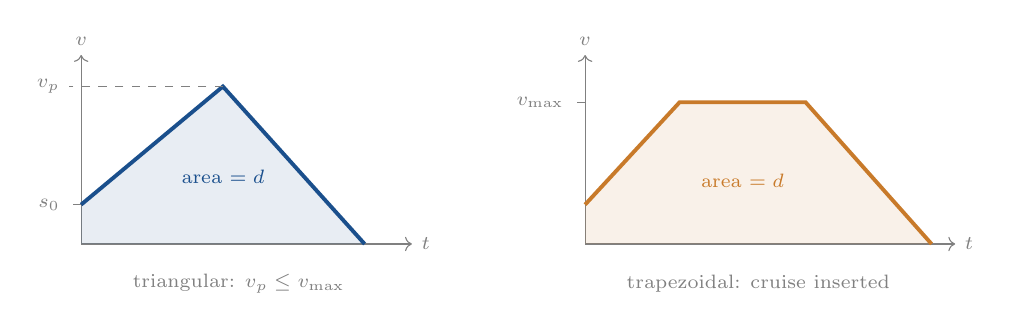
\begin{tikzpicture}[scale=1]
  \begin{scope}
    \draw[->,gray] (0,0) -- (4.2,0) node[right,font=\scriptsize] {$t$};
    \draw[->,gray] (0,0) -- (0,2.4) node[above,font=\scriptsize] {$v$};
    \draw[BlueLink,line width=1.4pt] (0,0.5) -- (1.8,2.0) -- (3.6,0);
    \fill[BlueLink,opacity=0.10] (0,0.5) -- (1.8,2.0) -- (3.6,0) -- (0,0) -- cycle;
    \draw[dashed,gray] (0,0.5) -- (-0.15,0.5) node[left,font=\scriptsize] {$s_0$};
    \draw[dashed,gray] (1.8,2.0) -- (-0.15,2.0) node[left,font=\scriptsize] {$v_p$};
    \node[font=\scriptsize,BlueLink] at (1.8,0.85) {area $=d$};
    \node[font=\scriptsize,gray] at (2.0,-0.5) {triangular: $v_p \le v_{\max}$};
  \end{scope}
  \begin{scope}[xshift=6.4cm]
    \draw[->,gray] (0,0) -- (4.7,0) node[right,font=\scriptsize] {$t$};
    \draw[->,gray] (0,0) -- (0,2.4) node[above,font=\scriptsize] {$v$};
    \draw[WarnRule,line width=1.4pt] (0,0.5) -- (1.2,1.8) -- (2.8,1.8) -- (4.4,0);
    \fill[WarnRule,opacity=0.10] (0,0.5) -- (1.2,1.8) -- (2.8,1.8) -- (4.4,0) -- (0,0) -- cycle;
    \draw[dashed,gray] (0,1.8) -- (-0.15,1.8) node[left,font=\scriptsize] {$v_{\max}$};
    \node[font=\scriptsize,WarnRule] at (2.0,0.8) {area $=d$};
    \node[font=\scriptsize,gray] at (2.2,-0.5) {trapezoidal: cruise inserted};
  \end{scope}
\end{tikzpicture}
\end{center}

\paragraph{Triangular case.} With peak $v_p$, using $v^2 = v_0^2 + 2a\Delta d$ on each leg:
\[
  d = \frac{v_p^2 - s_0^2}{2a_{\max}} + \frac{v_p^2}{2a_{\max}} = \frac{2v_p^2 - s_0^2}{2a_{\max}}
  \;\Longrightarrow\;
  \boxed{\;v_p = \sqrt{a_{\max}d + \tfrac12 s_0^2}\;}
\]
\begin{equation}
\label{eq:tri}
  T = \frac{v_p - s_0}{a_{\max}} + \frac{v_p}{a_{\max}} = \frac{2v_p - s_0}{a_{\max}} .
\end{equation}

\paragraph{Trapezoidal case.} If $v_p > v_{\max}$, cap it and insert a cruise:
\begin{equation}
\label{eq:trap}
  T = \frac{v_{\max}-s_0}{a_{\max}}
      + \frac{\big[d - d_{\text{acc}} - d_{\text{dec}}\big]_+}{v_{\max}}
      + \frac{v_{\max}}{a_{\max}} .
\end{equation}

The potential is
\begin{equation}
\label{eq:phibrake}
  \boxed{\;\varphi_{\text{brake}}(s) = -\,T\big(d_{\text{geo}}(x,y),\ |v|\big)\;}
\end{equation}
which is exactly \code{src/shaping/braking\_potential.py}:

\begin{lstlisting}
def bangbang_time(d, s0, v_max, a_max):
    d  = max(0.0, float(d))
    s0 = min(abs(float(s0)), v_max)
    peak = np.sqrt(a_max * d + 0.5 * s0 * s0)  # solves (2p^2-s0^2)/2a = d
    if peak <= v_max:
        return (2.0 * peak - s0) / a_max
    d_acc = (v_max * v_max - s0 * s0) / (2.0 * a_max)
    d_dec = v_max * v_max / (2.0 * a_max)
    return ((v_max - s0) / a_max
            + max(0.0, d - d_acc - d_dec) / v_max
            + v_max / a_max)
\end{lstlisting}

\subsection{The whole idea in one line}

Set $d=0$. Then $v_p = s_0/\sqrt2$ and
\begin{equation}
\label{eq:atgoal}
  T(0, v) = \frac{2(v/\sqrt2) - v}{a_{\max}} = \frac{(\sqrt2 - 1)v}{a_{\max}} > 0
  \qquad\text{for } v > 0 .
\end{equation}

\begin{keybox}
\textbf{Sitting on your goal while still moving is not free.} You have to shed that speed,
and shedding it costs time. $\varphi_{\text{dij}}$ says a robot parked on the goal at top
speed is finished. $\varphi_{\text{brake}}$ says it still owes
$(\sqrt2-1)(0.5)/0.25 = 0.83$ seconds.

That is the contribution, in one equation.
\end{keybox}

\subsection{Admissibility, and where it is loose}

\begin{proposition}
$T(d_{\text{geo}},|v|)$ lower-bounds the true minimum time-to-go; equivalently
$\varphi_{\text{brake}} \ge V^*$, i.e. the potential is optimistic.
\end{proposition}

Three relaxations, each of which can only reduce the estimate: $d_{\text{geo}}$ lower-bounds
the arclength of any feasible path; we take $s_0 = |v|$ rather than the component along the
path, crediting the robot with all its speed being useful; and curvature is ignored entirely,
though a real unicycle cannot turn tighter than $\rho = 1$\,m.

\begin{warnbox}
\textbf{Tightness has a documented hole.} When $d < v^2/(2a_{\max})$ --- the robot is closer
to the goal than its own braking distance --- it \emph{cannot} cover $d$ and still stop; it
must overshoot and come back. $T$ strictly under-estimates there. Admissibility is
unaffected (a heuristic may under-estimate) but the bound is not tight on the final approach.
Asserted and checked in \code{tests/test\_shaping\_gap.py}.
\end{warnbox}

\subsection{Does it generalise past the unicycle?}

A fair question, since a claim resting on one robot is not a principle.

\paragraph{Admissibility survives for holonomic robots.} With $\ddot\bp = \ba$,
$\|\ba\|\le a_{\max}$, Cauchy--Schwarz gives
$d\|\bv\|/dt = (\bv\cdot\ba)/\|\bv\| \le \|\ba\| \le a_{\max}$, so speed still cannot change
faster than $a_{\max}$ and the bang-bang time remains valid.

\paragraph{Tightness collapses.} A holonomic robot changes \emph{direction} without shedding
speed, so it never pays the turn-around cost. Measured error of Eq.~\ref{eq:phibrake} against
the true holonomic cost-to-go: $0\%$ with velocity toward the goal, $12\%$ perpendicular,
$36\%$ pointing away.

\paragraph{How to read that.} The non-holonomic unicycle always sits in the tight case --- it
cannot translate sideways, so speed in the wrong direction genuinely must be undone. That is
a \emph{feature} of the claim: the potential is exactly tight for the robots whose dynamics
make the problem hard, and loose for the ones where it was easier anyway.

%======================================================================
\section{Where the Theory and the Code Disagree}
\label{sec:gammabug}
%======================================================================

Now the bill for Section~\ref{sec:env}'s observation that PBRS violates the
environment/algorithm split.

$F$ contains $\gamma$, and $F$ is computed inside the environment when the reward is
assembled. So the environment needs a number that belongs to the algorithm. Our code
resolves this by giving the environment its \emph{own} $\gamma$:

\begin{lstlisting}
# src/env/multiagent_nav.py:45
self.gamma = cfg.shaping.gamma            # from conf/shaping/*.yaml
# src/env/multiagent_nav.py:212
rewards[agent] += self.shaping_scale * self.potentials[i].shaping(
    prev_states[i], self._states[i], self._goals[i], self.gamma)
\end{lstlisting}

and the two files disagree:

\begin{center}
\small
\begin{tabular}{llr}
\toprule
\textbf{Constant} & \textbf{File} & \textbf{Value} \\
\midrule
$\gamma_{\text{shape}}$ & \code{conf/shaping/braking.yaml} (and every other shaping file) & $1.00$ \\
$\gamma_{\text{learn}}$ & \code{conf/train/ppo\_default.yaml} & $0.99$ \\
\bottomrule
\end{tabular}
\end{center}

\begin{warnbox}
\textbf{Theorem 1 therefore does not cover our configuration.} It requires the $\gamma$ in
$F$ to be the learner's discount. We compute $F = \varphi(s')-\varphi(s)$ while optimising a
$0.99$-discounted return.

\textbf{It is deliberate, and the reason is quantitative.} With
$\gamma_{\text{shape}} = \gamma_{\text{learn}} = 0.99$, an agent that does nothing collects
\[
  F_{\text{idle}} = k(1-\gamma)|\varphi(s)| = 8.0 \times 0.01 \times 8.0 = +0.64 \ \text{per step},
\]
using $k=8.0$ and the measured $\varphi \approx -8.0$\,s at the \code{swap2} start, against
a time penalty of $-0.01$. \textbf{Standing still would pay sixty-four times better than the
penalty for standing still.} Setting $\gamma_{\text{shape}} = 1$ makes it exactly zero.
Whoever made this choice hit a real problem and solved it by breaking the theorem.
\end{warnbox}

\paragraph{What survives.} Precision matters, because a reviewer who knows PBRS will check.

\begin{itemize}[leftmargin=1.4em,itemsep=3pt]
\item \textbf{No reward hacking --- survives.} With $\gamma_{\text{shape}}=1$,
      $\sum_t[\varphi(s_{t+1})-\varphi(s_t)] = \varphi(s_T)-\varphi(s_0)$ depends only on
      endpoints, so shaping around any \emph{cycle} is exactly zero. This is the property we
      most need, and we still have it.
\item \textbf{Invariance for an undiscounted objective --- survives.} Read the objective as
      undiscounted finite-horizon total reward and $\gamma_{\text{shape}}=1$ is the
      \emph{correct} choice, with Theorem 1 applying exactly.
\item \textbf{Invariance for the $\gamma=0.99$ objective we actually optimise --- does not.}
      The discount breaks the telescoping, the shaping is no longer a constant offset, and it
      \emph{can} change the optimal policy. Direction and size of that bias are
      \textbf{not currently measured}.
\end{itemize}

\begin{keybox}
\textbf{How to write this honestly.} Do not cite Ng, Harada and Russell as though the
guarantee covers this implementation. Either state the objective as undiscounted and use
$\gamma_{\text{shape}}=1$ consistently --- cheap and defensible, it merely has to be
\emph{said} --- or set $\gamma_{\text{shape}} = \gamma_{\text{learn}}$ and drop $k$ until
$F_{\text{idle}}$ is small against the step penalty, accepting a far weaker shaping signal.

Note also the interaction with \S\ref{sec:trunc}: PBRS's compensation argument assumes
episodes end properly, and treating every timeout as a true terminal damages it further.
\textbf{Fix the truncation bug first, then decide on $\gamma_{\text{shape}}$.}
\end{keybox}
\part{What Happened}

%======================================================================
\section{First: Does the Gap Even Exist?}
\label{sec:stagea}
%======================================================================

Before training anything, a cheaper question. Part III argued that a position-only potential
must be wrong for a second-order robot. \emph{How wrong?} If the answer is ``negligibly'',
the project is over and we have saved ourselves a month.

Method: build a discrete lattice over $(x,y,\theta,v,\omega)$, run exact value iteration to
get $V^*$ in time units, and compare against the position-only estimate. Then sweep the
physically meaningful knob --- $d_{\text{brake}}$ --- by varying $v_{\max}$ and $a_{\max}$
independently.

\begin{center}
\small
\begin{tabular}{rrrrr}
\multicolumn{5}{c}{\textbf{Sweep A: vary $v_{\max}$, hold $a_{\max}=0.25$}}\\
\toprule
$v_{\max}$ & $d_{\text{brake}}$ & $\rho_{\text{brake}}$ & median gap & gap$/V$ \\
\midrule
0.25 & 0.125 & 0.62  & 1.050 & 0.088 \\
0.50 & 0.500 & 2.50  & 1.050 & 0.125 \\
0.75 & 1.125 & 5.62  & 1.750 & 0.333 \\
1.00 & 2.000 & 10.00 & 2.275 & 0.406 \\
\bottomrule
\multicolumn{5}{l}{\footnotesize $\text{corr}(d_{\text{brake}},\text{gap}) = 0.978$}
\end{tabular}
\qquad
\begin{tabular}{rrrr}
\multicolumn{4}{c}{\textbf{Sweep B: vary $a_{\max}$, hold $v_{\max}=0.5$}}\\
\toprule
$a_{\max}$ & $d_{\text{brake}}$ & mean gap & gap$/V$ \\
\midrule
0.500 & 0.250 & 0.655 & 0.117 \\
0.357 & 0.350 & 0.937 & 0.149 \\
0.286 & 0.437 & 0.937 & 0.149 \\
0.214 & 0.583 & 2.577 & 0.335 \\
0.143 & 0.875 & 2.577 & 0.335 \\
\bottomrule
\multicolumn{4}{l}{\footnotesize $\text{corr}(d_{\text{brake}},\text{gap}) = 0.886$}
\end{tabular}
\end{center}

At the benchmark's own parameters the position-only potential is wrong by $12.5\%$ of the
value function, and the error scales cleanly with braking distance in \emph{both} sweeps.
The gap is real, and it is controlled by the physical quantity the theory says controls it.

\begin{warnbox}
\textbf{This measurement took five attempts, and one of them printed a confident false
verdict.} Each bug below silently invalidated the previous result:
\begin{enumerate}[leftmargin=1.6em,itemsep=1pt]
\item $\Delta t \cdot v_{\max} = 0.05$\,m of travel per step against a $0.217$\,m cell:
      every transition was a self-loop. Fixed with held motion primitives.
\item The same defect on the velocity axes.
\item Sweeping $a_{\max}$ changed the velocity resolution row by row, so rows were not
      comparable. \textbf{This is what produced a printed verdict of ``S1 FALSIFIED''.}
\item The median is quantised onto the lattice, so it cannot support a monotonicity test.
      Switched to the mean; the log now says so.
\item A bang-off-bang action set made velocity resolution proportional to $a_{\max}$,
      yielding a $V^*$ that \emph{decreased} as more acceleration became available --- which
      is physically impossible.
\end{enumerate}
\textbf{The fix that mattered was structural, not any individual patch.} The script now runs
a hard self-test --- \emph{does more acceleration ever cost more time?} --- and
\textbf{refuses to print any gap number} if the answer is yes. Both logs show that test
passing on every adjacent pair of rows.

A discretised experiment that cannot detect its own discretisation error is not evidence. We
learned that the expensive way.
\end{warnbox}

%======================================================================
\section{One Robot: a Clean Win}
\label{sec:swap1}
%======================================================================

Before two robots, one. \code{swap1\_unicycle2} is the same benchmark instance with a single
robot driving three metres in a straight line. No coordination, no other agent --- purely a
test of whether the potential improves \emph{control quality}.

$400$k steps, seed $0$, $16$ parallel environments, $50$ evaluation episodes. Analytic
optimum: $76$ steps.

\begin{center}
\small
\begin{tabular}{lrrrr}
\toprule
& \textbf{success} & \textbf{crashes} & \textbf{collisions/ep} & \textbf{steps to goal} \\
\midrule
\code{dijkstra} (deterministic) & $100.0\%$ & $0.0\%$ & $0.0$ & $104.0$ \\
\code{braking}\ \ (deterministic) & $100.0\%$ & $0.0\%$ & $0.0$ & $\mathbf{70.0}$ \\
\midrule
\code{dijkstra} (stochastic)    & $100.0\%$ & $0.0\%$ & $0.0$ & $105.5$ \\
\code{braking}\ \ (stochastic)    & $100.0\%$ & $0.0\%$ & $0.4$ & $82.8$ \\
\bottomrule
\end{tabular}
\end{center}

\begin{keybox}
\textbf{$70$ steps against $104$: a $33\%$ reduction in completion time, at identical
$100\%$ success and zero collisions.}
\end{keybox}

The behaviour probe explains \emph{why}, which matters more than the headline:

\begin{center}
\small
\begin{tabular}{lrrrr}
\toprule
& \textbf{path length} & \textbf{mean $v$} & \textbf{mean $|v|$} & \textbf{\% reversing} \\
\midrule
\code{dijkstra} & $3.44$ m & $+0.138$ & $0.329$ & $34\%$ \\
\code{braking}  & $3.01$ m & $+0.426$ & $0.426$ & $\mathbf{0\%}$ \\
\bottomrule
\end{tabular}
\end{center}

The task is $3.00$\,m. The braking agent drives $3.01$\,m --- essentially the straight line
--- at $85\%$ of top speed, and never once reverses. The baseline drives $3.44$\,m, spends a
third of its time in reverse, and averages two-thirds of top speed.

That reversing figure is the tell, and it is Eq.~\ref{eq:atgoal} showing up in behaviour. A
position-only potential rewards \emph{being near} the goal, so an agent that overshoots is
rewarded for backing up; it learns overshoot-and-correct because nothing in its reward ever
told it that arriving fast is a debt. The velocity-aware potential charges that debt up
front, and the resulting behaviour is a clean single-pass approach.

\begin{keybox}
\textbf{Sanity check on the 70.} The analytic optimum is $76$ steps \emph{ending at rest}.
Beating it is not a bug: the goal gate accepts $|v| < 0.4$, so the agent legitimately skips
the final braking phase. It is exploiting a loose gate, correctly --- and the gate is the
benchmark's, not ours.
\end{keybox}

%======================================================================
\section{Two Robots: a Wall}
\label{sec:swap2}
%======================================================================

Same everything. Two robots, head-on, on the same line. Fifty evaluation episodes.

\begin{center}
\small
\begin{tabular}{lrr}
\toprule
& \textbf{success} & \textbf{collisions/ep (det.)} \\
\midrule
\code{dijkstra} & $0.0\%$ & $44$ \\
\code{braking}  & $0.0\%$ & $11$ \\
\bottomrule
\end{tabular}
\end{center}

Both fail completely. It is tempting to read $11 < 44$ as our method being four times safer.
The behaviour probe says otherwise:

\begin{center}
\small
\begin{tabular}{lr}
\toprule
& \textbf{closest approach} \\
\midrule
\code{dijkstra} & $0.04$ m --- goes for the gap \\
\code{braking}  & $1.08$ / $2.02$ m --- stops far away and waits \\
\bottomrule
\end{tabular}
\end{center}

\begin{warnbox}
\textbf{The braking agent's low collision count is timidity, not skill.} It stops one to two
metres out and waits for a gap that never comes. That is not a partial solution; it is a
different failure mode. A collision-count comparison between two agents that both fail
$100\%$ of the time is not a meaningful ranking and must not be presented as one.
\end{warnbox}

\paragraph{Why this is the interesting result.} Section~\ref{sec:swap1} isolates control
quality, and the potential wins decisively. This section adds exactly one thing --- a
symmetric conflict --- and both methods collapse to zero.

So the binding constraint in multi-robot kinodynamic navigation is \textbf{not} the quality
of the cost-to-go estimate. Improving $\varphi$ further will not fix \code{swap2}. Something
else is in the way, and the next section is about our first, wrong, guess at what it was.

%======================================================================
\section{Things We Believed That Were Wrong}
\label{sec:refuted}
%======================================================================

An account that lists only what worked is not an account. Three beliefs, and the evidence
that removed them.

\subsection{Refuted: ``the commitment horizon breaks credit assignment''}

\textbf{The claim.} Reciprocal avoidance requires committing to a yield roughly
$\tau \approx d_{\text{brake}}/v$ before contact. That delay between action and consequence
is what makes credit assignment hard, and it is the mechanism behind the failure.

It sounded right. It was constructed by us, not drawn from any paper. Three checks killed
it.

\begin{enumerate}[leftmargin=1.8em,itemsep=5pt]
\item \textbf{No literature support.} The delayed-reward survey \code{arXiv:2312.01072}
      offers no quantitative law relating delay to learning hardness. The mechanism had no
      source.

\item \textbf{The arithmetic refutes it.} Recall $\gamma\lambda = 0.9405$ from
      Section~7.1. The GAE weight at $\tau = 20$ steps is
      \[
        (\gamma\lambda)^{20} = 0.293 ,
      \]
      whereas the delays that genuinely break credit assignment --- $200$ steps in an Atari
      game --- carry weight $(\gamma\lambda)^{200} = 4.7\times10^{-6}$. A weight of $0.29$ is
      a \emph{strong} learning signal. \textbf{Twenty steps is short for RL, not long.}

\item \textbf{Direct measurement refutes it.} We instrumented episodes for first ICS entry
      against first collision:
      \begin{center}
      \small
      \begin{tabular}{lccc}
      \toprule
       & \textbf{enters ICS} & \textbf{collides} & \textbf{actual $\tau$} \\
      \midrule
      \code{dijkstra} & step $30$ & step $39$ & $9$ steps, GAE weight $0.58$ \\
      \code{braking}  & \textbf{never} & step $88$ & --- \\
      \bottomrule
      \end{tabular}
      \end{center}
      The baseline's real commitment horizon is nine steps, carrying more than half credit
      weight. And the braking agent \textbf{never enters an inevitable collision state at
      all} and still collides --- so its failures cannot be caused by late commitment in any
      sense.
\end{enumerate}

\begin{keybox}
\textbf{Conclusion.} The failure on \code{swap2} is not about \emph{timing}. It is about
\textbf{symmetry and yielding}: two identical agents, identically shaped, with uncorrelated
exploration noise, have no mechanism for agreeing who goes first. Part V takes that up.
\end{keybox}

\begin{warnbox}
\textbf{And the diagnostic that produced check 3 was itself wrong on its first run.} It read
\code{v.get("collisions", 0)} from the per-step info dictionary --- but \code{collisions} is
populated only in \code{info["episode"]} at episode end. The key was always absent, the
default $0$ always returned, and the script reported ``no collisions anywhere''. A clean
false finding produced by a defaulting dictionary lookup. Fixed by tracking
\code{env.\_collision\_count} deltas directly.
\end{warnbox}

\subsection{Corrected: ``speed-seeking is a flaw of the braking potential''}

An intermediate analysis claimed the braking agent's wall contacts revealed a defect in the
potential --- that it induces reckless speed-seeking. It does not. The agent was operating
near the dynamic limit, which is the potential working as designed, and it was being judged
on \emph{training-time} success under an exploration noise of $\sigma = 0.30$ against
$a_{\max} = 0.25$. That measurement is structurally biased against any method that operates
near the limit. The deterministic evaluation, once run, showed $100\%$ success and zero
collisions.

\subsection{Corrected: a premature recommendation to abort a run}

At $100$k steps the braking run showed rising collisions and was described as
``monotonically degrading'', with a recommendation to kill it. Collisions recovered from
$49$ to $5$ by $200$k, and the final result was the $33\%$ win of
Section~\ref{sec:swap1}. The recommendation was withdrawn and both runs were allowed to
finish.

\begin{keybox}
\textbf{The common thread.} Every one of these came from reading a partial or
mis-instrumented signal and forming a confident conclusion before the measurement was sound.
The countermeasure that actually worked is the one now built into
\code{scripts/shaping\_gap.py}: a self-test that \emph{refuses to emit numbers} when its own
validity precondition fails. That pattern is worth copying into every diagnostic we write
from here on.
\end{keybox}
\part{Where This Goes}

%======================================================================
\section{What We Actually Know}
%======================================================================

\begin{center}
\begin{tabular}{p{7.4cm}p{6.8cm}}
\toprule
\textbf{Established} & \textbf{Evidence} \\
\midrule
Position-only potentials are wrong for second-order robots --- $12.5\%$ of $V^*$ at
benchmark parameters, scaling with $d_{\text{brake}}$ &
Stage A, two sweeps, correlations $0.978$ / $0.886$, with a passing self-test \\
\addlinespace
A velocity-aware potential cuts completion time $33\%$ at equal success, single robot &
\code{swap1}, $50$ episodes, $104 \to 70$ steps \\
\addlinespace
Better cost-to-go does \emph{not} solve symmetric two-robot conflict &
\code{swap2}, both potentials $0\%$ \\
\addlinespace
The failure is not a credit-assignment-delay problem &
Three independent refutations, \S\ref{sec:refuted} \\
\addlinespace
Decentralised RL under true second-order dynamics is an unoccupied niche &
Action-space audit of the primary RL collision-avoidance papers \\
\bottomrule
\end{tabular}
\end{center}

\begin{keybox}
Read as a whole: \textbf{we have a working contribution at the single-robot level and a
clean, well-diagnosed wall at the multi-robot level.} The wall is not where we first thought
it was, and finding that out cost three wrong hypotheses --- which is the ordinary price of
the method working.
\end{keybox}

%======================================================================
\section{The Symmetry Problem, Framed Properly}
\label{sec:symmetry}
%======================================================================

Strip \code{swap2} to its bones. Two agents approach head-on. Each chooses to \textsc{yield}
or \textsc{go}. Yielding costs time; if both go, they collide.

Under second-order dynamics the cost of yielding is not arbitrary --- it is \emph{derived}.
Shedding speed $v$ and recovering it costs
\[
  c(v) = \frac{v}{a_{\max}} = \frac{2\,d_{\text{brake}}}{v},
\]
whereas for a first-order robot $c(v) = 0$: yielding is free and the game is trivial.

This is a \textbf{Chicken} game whose payoff matrix is written by the robot's acceleration
bound. It has no pure symmetric equilibrium, and its mixed equilibrium gives a collision
probability of the form $(c/C)^2$, where $C$ is the collision cost.

\begin{keybox}
\textbf{Why this is the promising direction.} It converts ``our method failed'' into a
structural statement:

\emph{for a symmetric second-order encounter there is no deterministic symmetric policy that
avoids collision, and the residual collision rate at equilibrium is a function of
$a_{\max}$.}

That is a claim with content. It predicts a specific dependence on a physical parameter, and
it is falsifiable by sweeping that parameter. It also \emph{explains} the $0\%$ rather than
excusing it: two identical networks with identical shaping and uncorrelated noise are
precisely the symmetric-strategy case the game says cannot work.
\end{keybox}

%======================================================================
\section{Assessed and Not Adopted: DiRL}
\label{sec:dirl}
%======================================================================

\textbf{DiRL} --- Jothimurugan, Bansal, Bastani and Alur, \emph{Compositional Reinforcement
Learning from Logical Specifications}, NeurIPS 2021 (\code{arXiv:2106.13906}) --- splits a
complex task into high-level planning plus low-level learning. The task is written as a
logical specification; the specification compiles to an \textbf{abstract graph} whose
vertices are regions of state space and whose edges are sub-tasks; Dijkstra searches that
graph for a shortest plan; and edge costs are estimated \emph{lazily} --- when Dijkstra asks
for one, DiRL builds a reward function for that sub-task and trains a policy to measure it.
Sample complexity then scales roughly linearly in specification size. It is single-agent,
and targets continuous state and action spaces.

\begin{warnbox}
\textbf{We already run Dijkstra, and it is not the same Dijkstra.} Ours runs over the
\textbf{workspace occupancy grid} to build a distance field that becomes a shaping potential
(Eq.~\ref{eq:dijkstra}); every cell is a physical location. DiRL's runs over an
\textbf{abstract task graph} in which every edge is an entire sub-task needing its own
trained policy; every vertex is a symbolic milestone.

Same algorithm, entirely different object. Ours is a \emph{heuristic evaluator}; theirs is a
\emph{task sequencer}. Writing that treats ``we use Dijkstra'' as the shared idea is wrong.
\end{warnbox}

\subsection{As published, it does not apply}

\textbf{Our specification has size one.} \code{swap2} is a single reach-avoid task: get to
the goal, do not collide. There is no sequence of milestones to order, and DiRL's entire
payoff is sample complexity linear in specification size. Dijkstra over a one-edge graph
returns that edge.

\textbf{And it is single-agent.} The abstract graph is built over one agent's state space.
Nothing in the construction addresses two agents negotiating who yields --- which
\S\ref{sec:refuted} identified as our actual failure mode.

\subsection{The adaptation that would fit, and what it costs}

One version does hit the real problem. Our evidence says the failure is symmetry, and
symmetry-breaking is a \emph{discrete} decision --- exactly what a graph planner is for. So
build the abstract graph over \textbf{coordination modes} rather than workspace regions:

\begin{center}
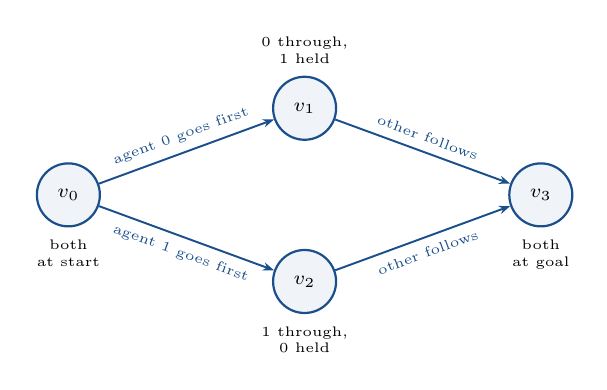
\begin{tikzpicture}[font=\scriptsize,
  v/.style={draw=BlueLink,fill=BoxBg,line width=0.8pt,circle,inner sep=3pt,minimum size=8mm},
  e/.style={-{Stealth[length=4pt]},line width=0.7pt,BlueLink}]
  \node[v] (v0) at (0,0)    {$v_0$};
  \node[v] (v1) at (3,1.1)  {$v_1$};
  \node[v] (v2) at (3,-1.1) {$v_2$};
  \node[v] (v3) at (6,0)    {$v_3$};
  \draw[e] (v0) -- node[above,sloped,font=\tiny]{agent 0 goes first} (v1);
  \draw[e] (v0) -- node[below,sloped,font=\tiny]{agent 1 goes first} (v2);
  \draw[e] (v1) -- node[above,sloped,font=\tiny]{other follows} (v3);
  \draw[e] (v2) -- node[below,sloped,font=\tiny]{other follows} (v3);
  \node[font=\tiny,align=center,below=1pt of v0] {both\\at start};
  \node[font=\tiny,align=center,above=1pt of v1] {0 through,\\1 held};
  \node[font=\tiny,align=center,below=1pt of v2] {1 through,\\0 held};
  \node[font=\tiny,align=center,below=1pt of v3] {both\\at goal};
\end{tikzpicture}
\end{center}

Dijkstra picks a branch, and \textbf{that breaks the symmetry by construction}. The
input/output change is small: the policy becomes sub-task conditioned,
$\pi_\theta(a \mid o, e)$, implemented by concatenating a one-hot edge identifier, so the
observation grows $13 \to 13+|E|$. Edge cost becomes measured expected completion time from
rollouts, and the planner outputs a sequence of edge policies.

The costs are less small:

\begin{center}
\small
\begin{tabular}{p{6.4cm}p{7.2cm}}
\toprule
\textbf{Problem} & \textbf{Consequence} \\
\midrule
Requires a \textbf{centralised} planner to pick the branch
  & Contradicts the decentralised premise. Survivable via centralised-training /
    decentralised-execution, but it must be stated, not glossed. \\
\addlinespace
$n!$ orderings for $n$ robots
  & No scaling claim past roughly three robots without restricting to pairwise conflicts. \\
\addlinespace
The graph is hand-authored
  & Fine for two robots; not a method. \\
\addlinespace
Abstract-graph Dijkstra is \textbf{dynamics-agnostic}
  & It does not depend on $a_{\max}$ at all --- \emph{orthogonal} to the kinodynamic
    contribution rather than a strengthening of it. \\
\bottomrule
\end{tabular}
\end{center}

That last row decides it. Our contribution is velocity-aware shaping for second-order
robots; DiRL is task decomposition. Bolted together they make two half-stories. And ``break
ties by agent index'' --- the obvious cheap symmetry-breaker --- is priority planning, which
is decades old.

\subsection{The one combination that is genuinely attractive}
\label{sec:dirlheur}

\begin{warnbox}
\textbf{What follows is our own construction, not a result from any paper, and untested.} It
is recorded as a hypothesis and must not be described as established.
\end{warnbox}

DiRL's dominant expense is edge-cost estimation --- it \emph{trains a policy} to discover
what an edge costs. Our bang-bang time $T(d,|v|)$ is an \textbf{analytic, admissible lower
bound} on exactly that quantity for a navigation edge, in closed form, at zero cost. Dijkstra
requires a lower bound to prune soundly. So the braking potential could \textbf{initialise
DiRL's lazy edge-cost estimates}, letting the planner skip training on edges a bound already
rules out.

That is a real interface --- the kinodynamic result \emph{serving} the planning result ---
rather than a bolt-on. It does not, by itself, fix symmetry.

\subsection{Recommendation}

\begin{keybox}
\textbf{Do not pivot to DiRL.} Keep it in related work and record \S\ref{sec:dirlheur} as
future work. Our specification has no compositional structure to exploit, the algorithm is
single-agent, and the adaptation needed is substantial enough that ``we applied DiRL'' would
misdescribe the work.
\end{keybox}

%======================================================================
\section{Defects, and the Order to Fix Them}
\label{sec:defects}
%======================================================================

Ranked by how much each would change a published result.

\begin{enumerate}[leftmargin=1.8em,itemsep=6pt]

\item \textbf{Neighbour velocity is absent from the observation.} \emph{(Critical.)} For a
second-order reciprocal-avoidance problem this is close to disqualifying --- the agent cannot
compute time-to-collision or a braking margin, because the quantity is not in its input. Two
lines in \code{src/obs/full\_state.py}. \textbf{First experiment to run.}

\item \textbf{$\gamma_{\text{shape}} = 1.0 \ne \gamma_{\text{learn}} = 0.99$.}
\emph{(High --- a correctness claim, not a performance one.)} \S\ref{sec:gammabug}.
Deliberate and well-motivated, but it forfeits the Ng--Harada--Russell guarantee for the
objective we actually optimise. Cheap to resolve in the writing; must not be left implicit.

\item \textbf{\code{time\_limit\_bootstrap} is unset.} \emph{(High, one line.)}
\S\ref{sec:trunc}. Because \code{swap2} succeeds $0\%$ of the time, this biases the critic on
essentially every trajectory.

\item \textbf{Exploration noise exceeds the action range.} \emph{(High.)}
$\sigma = 0.301$ against $a_{\max} = 0.25$, state-independent, and never logged. Lower the
initialisation or make \code{log\_std} a network head.

\item \textbf{Critic sees only local observations.} \emph{(Medium; deliberate.)} It is what
makes the algorithm IPPO, but it means the $0\%$ cannot distinguish ``shaping insufficient''
from ``independent learning insufficient''. A MAPPO ablation on the already-exposed $\R^{26}$
state separates them cheaply.

\item \textbf{A unimodal Gaussian cannot represent a bang-bang optimum.} \emph{(Medium.)}

\item \textbf{Fixed-width neighbour block.} \emph{(Low now, blocking later.)} Prevents
transfer across robot counts, so no scaling result without an architecture change.
\end{enumerate}

\subsection{The decisive experiment}

\begin{keybox}
\textbf{Run the identical geometry with a first-order robot and a second-order robot.} Same
instance, same $v_{\max}$, same shaping, same algorithm, same seeds --- differing only in
whether the action is velocity or acceleration.

If the first-order version solves \code{swap2} and the second-order version does not, the
acceleration bound is established as the cause and \S\ref{sec:symmetry} gains an empirical
anchor. If both fail, the problem is symmetry alone and the kinodynamic framing is not the
story. \emph{Either outcome is publishable, and the experiment is cheap.}
\end{keybox}

\subsection{Ordered plan}

\begin{enumerate}[leftmargin=1.8em,itemsep=3pt]
\item Add neighbour velocity to the observation; re-run \code{swap2}. \emph{(Defect 1.)}
\item Decide and \emph{state} the $\gamma_{\text{shape}}$ convention. \emph{(Defect 2.)}
\item Set \code{time\_limit\_bootstrap = True}. \emph{(Defect 3.)}
\item Run first-order versus second-order on identical geometry.
\item Sweep $a_{\max}$ and test the predicted collision-rate dependence.
\item Run the MAPPO ablation.
\item Only then commit to a paper framing.
\end{enumerate}

\noindent DiRL is deliberately absent from this list: it is orthogonal to the kinodynamic
contribution and advances no step above.
\appendix
\part*{Appendices}
\addcontentsline{toc}{part}{Appendices}

%======================================================================
\section{Inputs and Outputs}
\label{app:io}
%======================================================================

\subsection{The whole pipeline}

\begin{center}
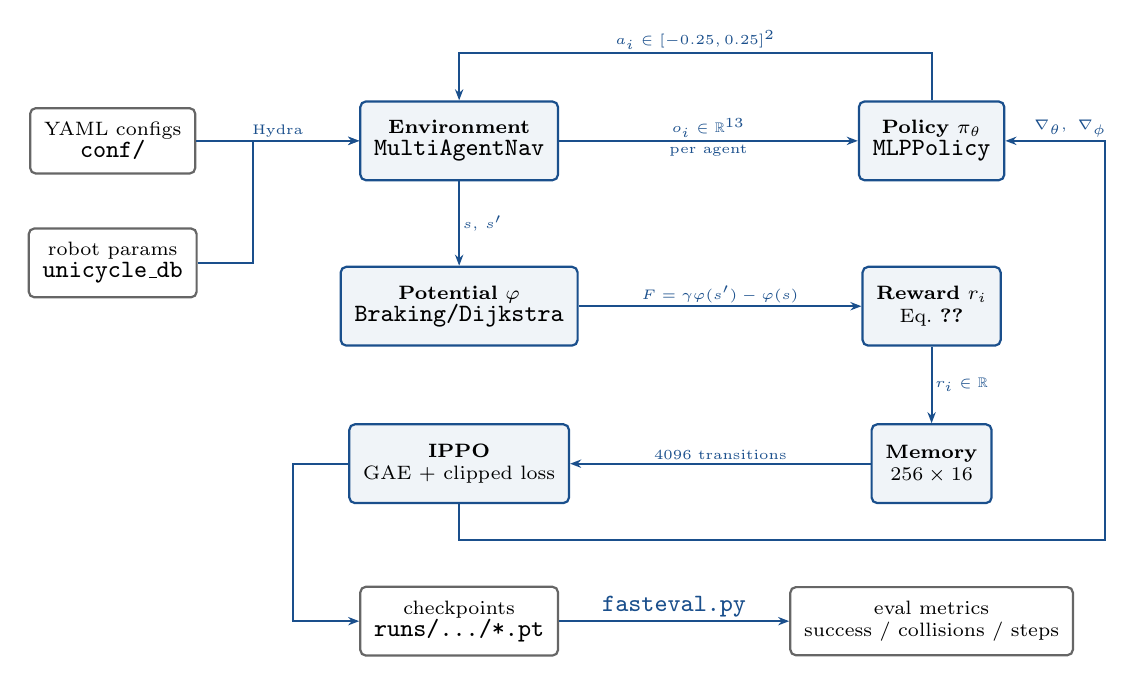
\begin{tikzpicture}[
  font=\scriptsize,
  box/.style={draw=BlueLink,fill=BoxBg,line width=0.8pt,rounded corners=2pt,
              inner sep=5pt,align=center,minimum height=10mm},
  ext/.style={draw=Gray60,fill=white,line width=0.8pt,rounded corners=2pt,
              inner sep=5pt,align=center,minimum height=8mm},
  fl/.style={-{Stealth[length=4pt]},line width=0.7pt,BlueLink},
  lbl/.style={font=\tiny,inner sep=1pt,fill=white}
]
\node[ext] (yaml) at (0,4.6)  {YAML configs\\\code{conf/}};
\node[ext] (rob)  at (0,3.05) {robot params\\\code{unicycle\_db}};
\node[box] (env) at (4.4,4.6)  {\textbf{Environment}\\\code{MultiAgentNav}};
\node[box] (pol) at (10.4,4.6) {\textbf{Policy} $\pi_\theta$\\\code{MLPPolicy}};
\node[box] (pot) at (4.4,2.5)  {\textbf{Potential} $\varphi$\\\code{Braking/Dijkstra}};
\node[box] (rew) at (10.4,2.5) {\textbf{Reward} $r_i$\\Eq.~\ref{eq:reward}};
\node[box] (ippo) at (4.4,0.5) {\textbf{IPPO}\\GAE + clipped loss};
\node[box] (mem)  at (10.4,0.5){\textbf{Memory}\\$256\times16$};
\draw[fl] (yaml) -- node[lbl,above]{Hydra} (env);
\draw[fl] (rob.east) -- ++(0.7,0) |- (env.west);
\draw[fl] (env) -- node[lbl,above]{$o_i\in\R^{13}$} node[lbl,below]{per agent} (pol);
\draw[fl] (pol.north) -- ++(0,0.6) -| node[lbl,above,pos=0.25]{$a_i\in[-0.25,0.25]^2$} (env.north);
\draw[fl] (env) -- node[lbl,right]{$s,\,s'$} (pot);
\draw[fl] (pot) -- node[lbl,above]{$F=\gamma\varphi(s')-\varphi(s)$} (rew);
\draw[fl] (rew) -- node[lbl,right]{$r_i\in\R$} (mem);
\draw[fl] (mem) -- node[lbl,above]{4096 transitions} (ippo);
\draw[fl] (ippo.south) -- ++(0,-0.45) -| (12.6,-0.45)
      -- (12.6,4.6) -- node[lbl,above,pos=0.35]{$\nabla_\theta,\ \nabla_\phi$} (pol.east);
\node[ext] (ckpt) at (4.4,-1.5) {checkpoints\\\code{runs/.../*.pt}};
\draw[fl] (ippo.west) -- ++(-0.7,0) |- (ckpt.west);
\node[ext] (metr) at (10.4,-1.5) {eval metrics\\success / collisions / steps};
\draw[fl] (ckpt) -- node[lbl,above]{\code{fasteval.py}} (metr);
\end{tikzpicture}
\end{center}

\subsection{Boundary by boundary}

\begin{center}
\footnotesize
\begin{tabular}{p{2.5cm}p{3.5cm}p{3.4cm}p{4.0cm}}
\toprule
\textbf{Boundary} & \textbf{Input} & \textbf{Output} & \textbf{Produced by} \\
\midrule
config $\to$ env & YAML tree & constructed env object & Hydra + \code{env/factory.py} \\
\addlinespace
env $\to$ policy & true state $s\in\R^{10}$ & $o_i \in \R^{13}$, \code{float32} & \code{obs/full\_state.py} \\
\addlinespace
policy $\to$ env & $o_i \in \R^{13}$ & $a_i \in [-0.25,0.25]^2$, m/s$^2$, rad/s$^2$ & \code{networks/policy.py} \\
\addlinespace
env internal & $\bx_t\in\R^5$, $\bu_t\in\R^2$ & $\bx_{t+1}$ after RK4, $\Delta t=0.1$\,s & robot model \\
\addlinespace
potential $\to$ reward & $s,s'$ (needs $x,y,v$) & scalar $F$ & \code{shaping/*.py} \\
\addlinespace
env $\to$ learner & --- & $r_i$, \code{terminated}, \code{truncated}, \code{info} & \code{multiagent\_nav.py} \\
\addlinespace
learner $\to$ disk & 4096 transitions/agent & weights, TensorBoard scalars & skrl IPPO \\
\addlinespace
disk $\to$ report & checkpoint \code{.pt} & success \%, collisions/ep, steps & \code{scripts/fasteval.py} \\
\bottomrule
\end{tabular}
\end{center}

\subsection{Three details that are easy to get wrong}

\paragraph{The observation is not the state.} The learner never sees $s\in\R^{10}$; it sees
$o_i\in\R^{13}$. And $13 \ne 10$ because the observation is a \emph{re-encoding}, not a
subset --- it adds derived quantities (bearings, wall distances) and drops others (the
neighbour's velocity). More numbers, less information.

\paragraph{The joint state is computed and then ignored.} The env exposes
\code{state\_spaces} $=\R^{26}$. IPPO never reads it. The MAPPO wiring is already in place.

\paragraph{\code{collisions} lives in two places.} Mid-episode the counter is internal,
as \code{env.\_collision\_count}. The key \code{"collisions"} appears \emph{only} inside
\code{infos[a]["episode"]}, and only at episode end. Reading it per-step therefore returns
$0$ for ever --- the bug behind the false finding in \S\ref{sec:refuted}.

\subsection{A run, end to end}

\begin{lstlisting}
INPUT   python main.py env=swap2_unicycle2 shaping=braking train.timesteps=400000
        `-- conf/config.yaml composes: approach, env, shaping, network, obs, init, train

OUTPUT  runs/braking_mlp_full_state/<timestamp>/
        |-- checkpoints/agent_50000.pt ... agent_400000.pt, best_agent.pt
        `-- events.out.tfevents.*            (TensorBoard scalars)

INPUT   python scripts/fasteval.py --checkpoint <path> --episodes 50
OUTPUT  success rate, crash rate, mean collisions/episode, mean steps on success
\end{lstlisting}

%======================================================================
\section{The Software Stack}
\label{app:tools}
%======================================================================

Versions are those installed in \code{.venv} at the time of writing.

\begin{center}
\footnotesize
\begin{tabular}{p{2.3cm}p{1.3cm}p{5.2cm}p{4.6cm}}
\toprule
\textbf{Tool} & \textbf{Version} & \textbf{What it does for us} & \textbf{What it does \emph{not} do} \\
\midrule
\textbf{Hydra} & 1.3.3
  & Composes the config tree from \code{conf/} --- one file per group, CLI overridable. Creates the run directory.
  & No runtime role after construction. \\
\addlinespace
\textbf{OmegaConf} & 2.3.1
  & The config object itself; used directly for the \code{a\_max\_override} merge.
  & Not a validator --- a typo in a key is silent. \\
\addlinespace
\textbf{PettingZoo} & 1.26.1
  & Defines the multi-agent API contract we implement: \code{ParallelEnv}, dict-in/dict-out stepping.
  & Supplies no environments we use, and no learning. Pure interface. \\
\addlinespace
\textbf{Gymnasium} & 1.3.0
  & The \code{Box} space objects declaring shapes and bounds.
  & Single-agent API; not used for stepping. \\
\addlinespace
\textbf{skrl} & 1.4.3
  & \textbf{The RL library.} IPPO, \code{RandomMemory}, \code{SequentialTrainer}, \code{RunningStandardScaler}, \code{KLAdaptiveLR}, model mixins, checkpointing, TensorBoard. Owns GAE and the clipped loss.
  & Owns nothing about the robot. Source of the \code{time\_limit\_bootstrap} defect. \\
\addlinespace
\textbf{PyTorch} & 2.12 & Networks, autodiff, optimiser, GPU. & --- \\
\addlinespace
\textbf{NumPy} & 2.2.6
  & \textbf{All environment physics.} RK4, collision geometry, the Dijkstra field, the bang-bang potential. Tensors appear only at the skrl boundary.
  & --- \\
\addlinespace
\textbf{dynobench} & (data)
  & Robot parameters. \code{unicycle2\_v0} copied verbatim into \code{conf/robot/}.
  & \textbf{Not a runtime dependency.} We re-implemented the model. \\
\addlinespace
\textbf{db-CBS} & (data)
  & Scenario geometry, ported into \code{conf/env/}.
  & Not installed. Its planner is a future baseline. \\
\addlinespace
matplotlib, Pillow & --- & Episode GIF rendering. & --- \\
pytest, ruff & --- & \code{tests/} (21 passing) and linting. & --- \\
\bottomrule
\end{tabular}
\end{center}

\begin{center}
\small
\begin{tabular}{p{6.4cm}p{7.4cm}}
\toprule
\textbf{Decision} & \textbf{Owned by} \\
\midrule
Robot dynamics, integration, bounds & \textbf{us} --- \code{src/robots/}, NumPy \\
What the agent can see & \textbf{us} --- \code{src/obs/full\_state.py} \\
Reward, goal test, termination & \textbf{us} --- \code{src/env/multiagent\_nav.py} \\
The shaping potential & \textbf{us} --- \code{src/shaping/} \ (\emph{the contribution}) \\
Network architecture & \textbf{us} --- \code{src/networks/} \\
GAE, PPO loss, adaptive LR, checkpointing & \textbf{skrl} \\
Multi-agent stepping contract & \textbf{PettingZoo} \\
Which config files load & \textbf{Hydra} \\
Robot constants and scenario geometry & \textbf{dynobench / db-CBS}, copied as data \\
\bottomrule
\end{tabular}
\end{center}

\begin{keybox}
\textbf{The short version.} We own the physics, the observation, the reward and the
potential. skrl owns the learning algorithm. PettingZoo owns the API shape. Hydra owns
configuration. The benchmark projects contribute \emph{numbers}, not code.

That matters for the paper: every claimed contribution lives in code we wrote, and every
number that makes the setup comparable to the literature comes from a published source
rather than from tuning.
\end{keybox}

%======================================================================
\section{Hyperparameters}
\label{app:hyper}
%======================================================================

\begin{center}
\small
\begin{tabular}{llp{7.4cm}}
\toprule
\textbf{Parameter} & \textbf{Value} & \textbf{Why} \\
\midrule
\code{timesteps}          & $1{,}000{,}000$ & trainer iterations; each advances all $16$ worlds one $\Delta t$ \\
\code{num\_envs}          & $16$      & parallel worlds; lower-variance gradient, denser reach signal \\
\code{rollouts}           & $256$     & $256\times16 = 4096$ transitions/agent per update \\
\code{mini\_batches}      & $8$       & minibatch $=512$ \\
\code{epochs}             & $3$       & $24$ gradient steps per update \\
\code{learning\_rate}     & $5\times10^{-5}$ & damps the reach-then-diverge oscillation \\
\code{max\_lr}            & $1\times10^{-4}$ & \textbf{scar tissue}: skrl's default $10^{-2}$ let the LR climb $200\times$ and detonate a converged policy \\
\code{min\_lr}            & $1\times10^{-5}$ & floor \\
\code{kl\_threshold}      & $0.01$    & trust region for the adaptive LR \\
\code{discount} $\gamma$  & $0.99$    & effective horizon $100$ steps $=10$\,s \\
\code{lambda\_} $\lambda$ & $0.95$    & GAE horizon $\approx16.8$ steps $\approx1.7$\,s \\
\code{clip\_ratio}        & $0.2$     & PPO clip \\
\code{entropy\_loss\_scale} & $0.01$  & steadier exploration \\
\code{value\_preprocessor}  & \textbf{off} & returns are bimodal ($0..{+}100$ vs $-500$); the running std swung and destabilised value loss \\
\code{clip\_predicted\_values} & \code{True} & damps critic swings \\
\code{seed}               & $42$      & \\
\midrule
\code{shaping.gamma}      & $1.0$     & \textbf{$\ne$ \code{discount}} --- see \S\ref{sec:gammabug} \\
\code{shaping\_scale} $k$ & $8.0$     & \\
\code{cell\_size}         & $0.1$\,m  & Dijkstra grid --- error budget in \S\ref{sec:disc} \\
\bottomrule
\end{tabular}
\end{center}

\begin{lstlisting}
per trainer timestep:
    16 worlds step in parallel (sub-envs auto-reset internally; `agents` always
    non-empty so the trainer never global-resets)
    each agent stores (o, a, log_pi, r, terminated, truncated, V(o)) in its OWN memory

every 256 timesteps:
    buffer = 256 x 16 = 4096 transitions per agent
    compute GAE(lambda=0.95, gamma=0.99) backwards over the buffer
    3 epochs x 8 minibatches = 24 gradient steps, minibatch = 512
        L = -min(rho*A, clip(rho, 0.8, 1.2)*A) + MSE(V, R) - 0.01*H[pi]
    KLAdaptiveLR: KL > 0.01 -> lr down; KL < 0.01 -> lr up; clamped [1e-5, 1e-4]
    clear memory
\end{lstlisting}

%======================================================================
\section{Source Map}
\label{app:src}
%======================================================================

\begin{center}
\footnotesize
\begin{tabular}{ll}
\toprule
\textbf{Path} & \textbf{Role} \\
\midrule
\code{src/env/multiagent\_nav.py}     & PettingZoo \code{ParallelEnv}; reward, termination, freeze-on-reach \\
\code{src/env/vec\_multiagent.py}     & $16$ independent worlds, internal auto-reset \\
\code{src/env/factory.py}             & builds env from Hydra config; \code{a\_max\_override} \\
\code{src/obs/full\_state.py}         & the $13$-d egocentric observation \\
\code{src/shaping/base.py}            & $F = \gamma\varphi(s') - \varphi(s)$ \\
\code{src/shaping/dijkstra\_potential.py} & baseline $\varphi = -d/v_{\max}$ \\
\code{src/shaping/braking\_potential.py}  & \textbf{ours}: $\varphi = -T_{\text{bangbang}}(d,|v|)$ \\
\code{src/networks/policy.py}         & Gaussian MLP, $\tanh$-squashed mean \\
\code{src/networks/value.py}          & critic MLP, takes \emph{local} obs \\
\code{src/approach/rl/train.py}       & skrl IPPO wiring \\
\code{conf/robot/unicycle\_db.yaml}   & dynobench \code{unicycle2\_v0}, verbatim \\
\code{conf/env/swap\{1,2\}\_unicycle2.yaml} & db-CBS instances, ported \\
\code{scripts/shaping\_gap.py}        & Stage A value iteration + self-test \\
\code{tests/test\_shaping\_gap.py}    & RK4 agreement; lower-bound vs tightness \\
\code{tests/test\_shaping.py}         & PBRS telescoping; the $\gamma$ convention \\
\bottomrule
\end{tabular}
\end{center}

%======================================================================
\section{Reading List}
\label{app:read}
%======================================================================

\begin{warnbox}
\textbf{Citation status is tracked explicitly.} This project has already produced one
fabricated citation --- ``Liu et al., RA-L 2017'' for what is in fact \emph{Liu, Atanasov,
Mohta and Kumar, IROS 2017} --- and one invented model name
(\code{unicycle\_second\_order\_0} is the db-CBS \emph{scenario} type string, not the
dynobench \emph{model} file, which is \code{unicycle2\_v0}). \textbf{Nothing below enters a
\code{.bib} until its metadata has been checked against the publisher record.}
\end{warnbox}

\begin{center}
\small
\begin{tabular}{p{6.2cm}p{4.4cm}p{3.0cm}}
\toprule
\textbf{Work} & \textbf{Why} & \textbf{Status} \\
\midrule
\multicolumn{3}{l}{\textit{Reward shaping}}\\
Ng, Harada, Russell --- \emph{Policy invariance under reward transformations}, ICML 1999
  & the PBRS theorem & confident \\
Wiewiora --- \emph{Potential-based shaping and Q-value initialization are equivalent}, JAIR 2003
  & why $\varphi \approx V^*$ is the target & confident \\
Devlin \& Kudenko --- multi-agent PBRS
  & does invariance survive with $>1$ learner? & \textbf{unverified} \\
\midrule
\multicolumn{3}{l}{\textit{Policy gradient}}\\
Schulman et al.\ --- PPO, \code{arXiv:1707.06347} & Eq.~\ref{eq:ppo} & confident \\
Schulman et al.\ --- GAE, \code{arXiv:1506.02438} & Eq.~\ref{eq:gae} & confident \\
de Witt et al.\ --- \code{arXiv:2011.09533} & IPPO vs MAPPO evidence & confident \\
\midrule
\multicolumn{3}{l}{\textit{Learned collision avoidance (all first-order)}}\\
Long et al., ICRA 2018 --- \code{arXiv:1709.10082} & the action-space gap & confident \\
Fan et al., IJRR --- \code{arXiv:1808.03841}       & same & confident \\
\midrule
\multicolumn{3}{l}{\textit{Kinodynamic planning (no learning)}}\\
Donald, Xavier, Canny, Reif --- \emph{Kinodynamic motion planning}, JACM 1993 & the original formulation & confident \\
Fraichard \& Asama --- \emph{Inevitable collision states}, Adv.\ Robotics 2004 & the ICS concept & confident \\
Liu, Atanasov, Mohta, Kumar, IROS 2017 --- \code{arXiv:1709.05401} & minimum-time heuristics & \textbf{corrected} \\
db-CBS & our benchmark source & \textbf{authors to verify} \\
K-CBS, K-ARC & the planning baselines to beat & \textbf{to verify} \\
\midrule
\multicolumn{3}{l}{\textit{Planning + learning (assessed, \S\ref{sec:dirl})}}\\
Jothimurugan, Bansal, Bastani, Alur --- \emph{Compositional RL from Logical
Specifications}, NeurIPS 2021, \code{arXiv:2106.13906} & DiRL & confident \\
\midrule
\multicolumn{3}{l}{\textit{Reciprocal avoidance}}\\
Fiorini \& Shiller --- velocity obstacles, IJRR 1998 & the geometric ancestor & confident \\
van den Berg, Guy, Lin, Manocha --- ORCA, ISRR 2011 & the first-order standard & confident \\
\bottomrule
\end{tabular}
\end{center}

\subsection{Process constraints on this project}

\begin{keybox}
\begin{itemize}[leftmargin=1.2em,itemsep=2pt]
\item \textbf{No quoted baseline numbers.} All baselines will be re-run in this environment
      rather than cited from their papers.
\item \textbf{Every citation verified before it enters the \code{.bib}.}
\item \textbf{IEEE-RAS AI policy.} AI cannot be an author. AI-generated content --- text,
      figures, or code --- must be disclosed in the acknowledgements, naming the system and
      the sections involved. Accepted papers are screened, including for hallucinated
      citations; violations are withdrawn from the programme and from IEEE Xplore with no
      refund of the registration fee.
\end{itemize}
\end{keybox}

\vspace{1em}
\noindent\rule{\linewidth}{0.4pt}
\vspace{0.3em}

\noindent\footnotesize\color{Gray60}
This report was drafted with AI assistance (Claude Opus 5) from the project source tree and
its logged experiment outputs, and is subject to author review before any of its content is
used in a submission. All quantitative values were read from \code{src/}, \code{conf/} and
\code{experiments/} at the time of writing rather than reproduced from memory. Items marked
\textbf{unverified} or \textbf{to verify} have not been checked against a publisher record
and must not be cited until they are.

\end{document}
